 \chapter{Introduction}
\label{cp.intro}

From ancient times to the modern day, astronomy has played an essential role in all cultures and eras.
Questions about the infinite cosmos and our place in it have intrigued great minds for millennia.
To answer these questions, astronomers construct instruments to record observational data from the universe and devise statistical methods to make inferences.
Each drop of cosmic data improves inference and takes us to the answers we seek.
However, until quite recently, astronomy has existed in a relatively data-poor environment. 
Using computers and sophisticated instruments, astronomers can now access massive datasets.
In response, some astronomers are turning to data-driven approaches to make inferences with the vast quantities of newly acquired data.
This section looks back at areas of astronomy that have recently seen significant data analysis improvements and have provided new insights into the nature of stars, planets, and even black holes.
This discussion will spark ideas and provide the impetus for the rest of the thesis.


\section{Observational HR-Diagrams through the ages}

\textbf{The first Observational HR-Diagram:}
In 1872, astronomers began recording spectroscopic data for thousands of stars in the Henry Draper Catalogue~\cite{Cannon:1918:AnHar}.
Antonia Maury, a female astronomer working in the Harvard observatory, noticed that some stars in the catalog were much brighter than other stars of the same color and sorted those brighter stars into a different category from their less-luminous brethren~\cite{1914_HR_data}. 
Several years later, Einjar Hertzpsrung, working on his star classification project in 1905, noticed the same thing as Maury: some stars had very similar colors but very different brightness~\cite{1914_HR_data}.
With more data available in 1913, Henry Norris Russell demonstrated the effect far more strikingly. 
Russell plotted the absolute magnitude against spectral type for Maury's stars, nearby stars with parallaxes measured at the time, stars from the open cluster Hyades, and several moving groups ($\sim200$ stars in total). 
This plot, an observational Hertzpsrung-Russel (HR) diagram, has been recreated with modern stellar data in Figure~\ref{fig:HR-diagrams}a.

\begin{figure}
\begin{center}
  \centerline{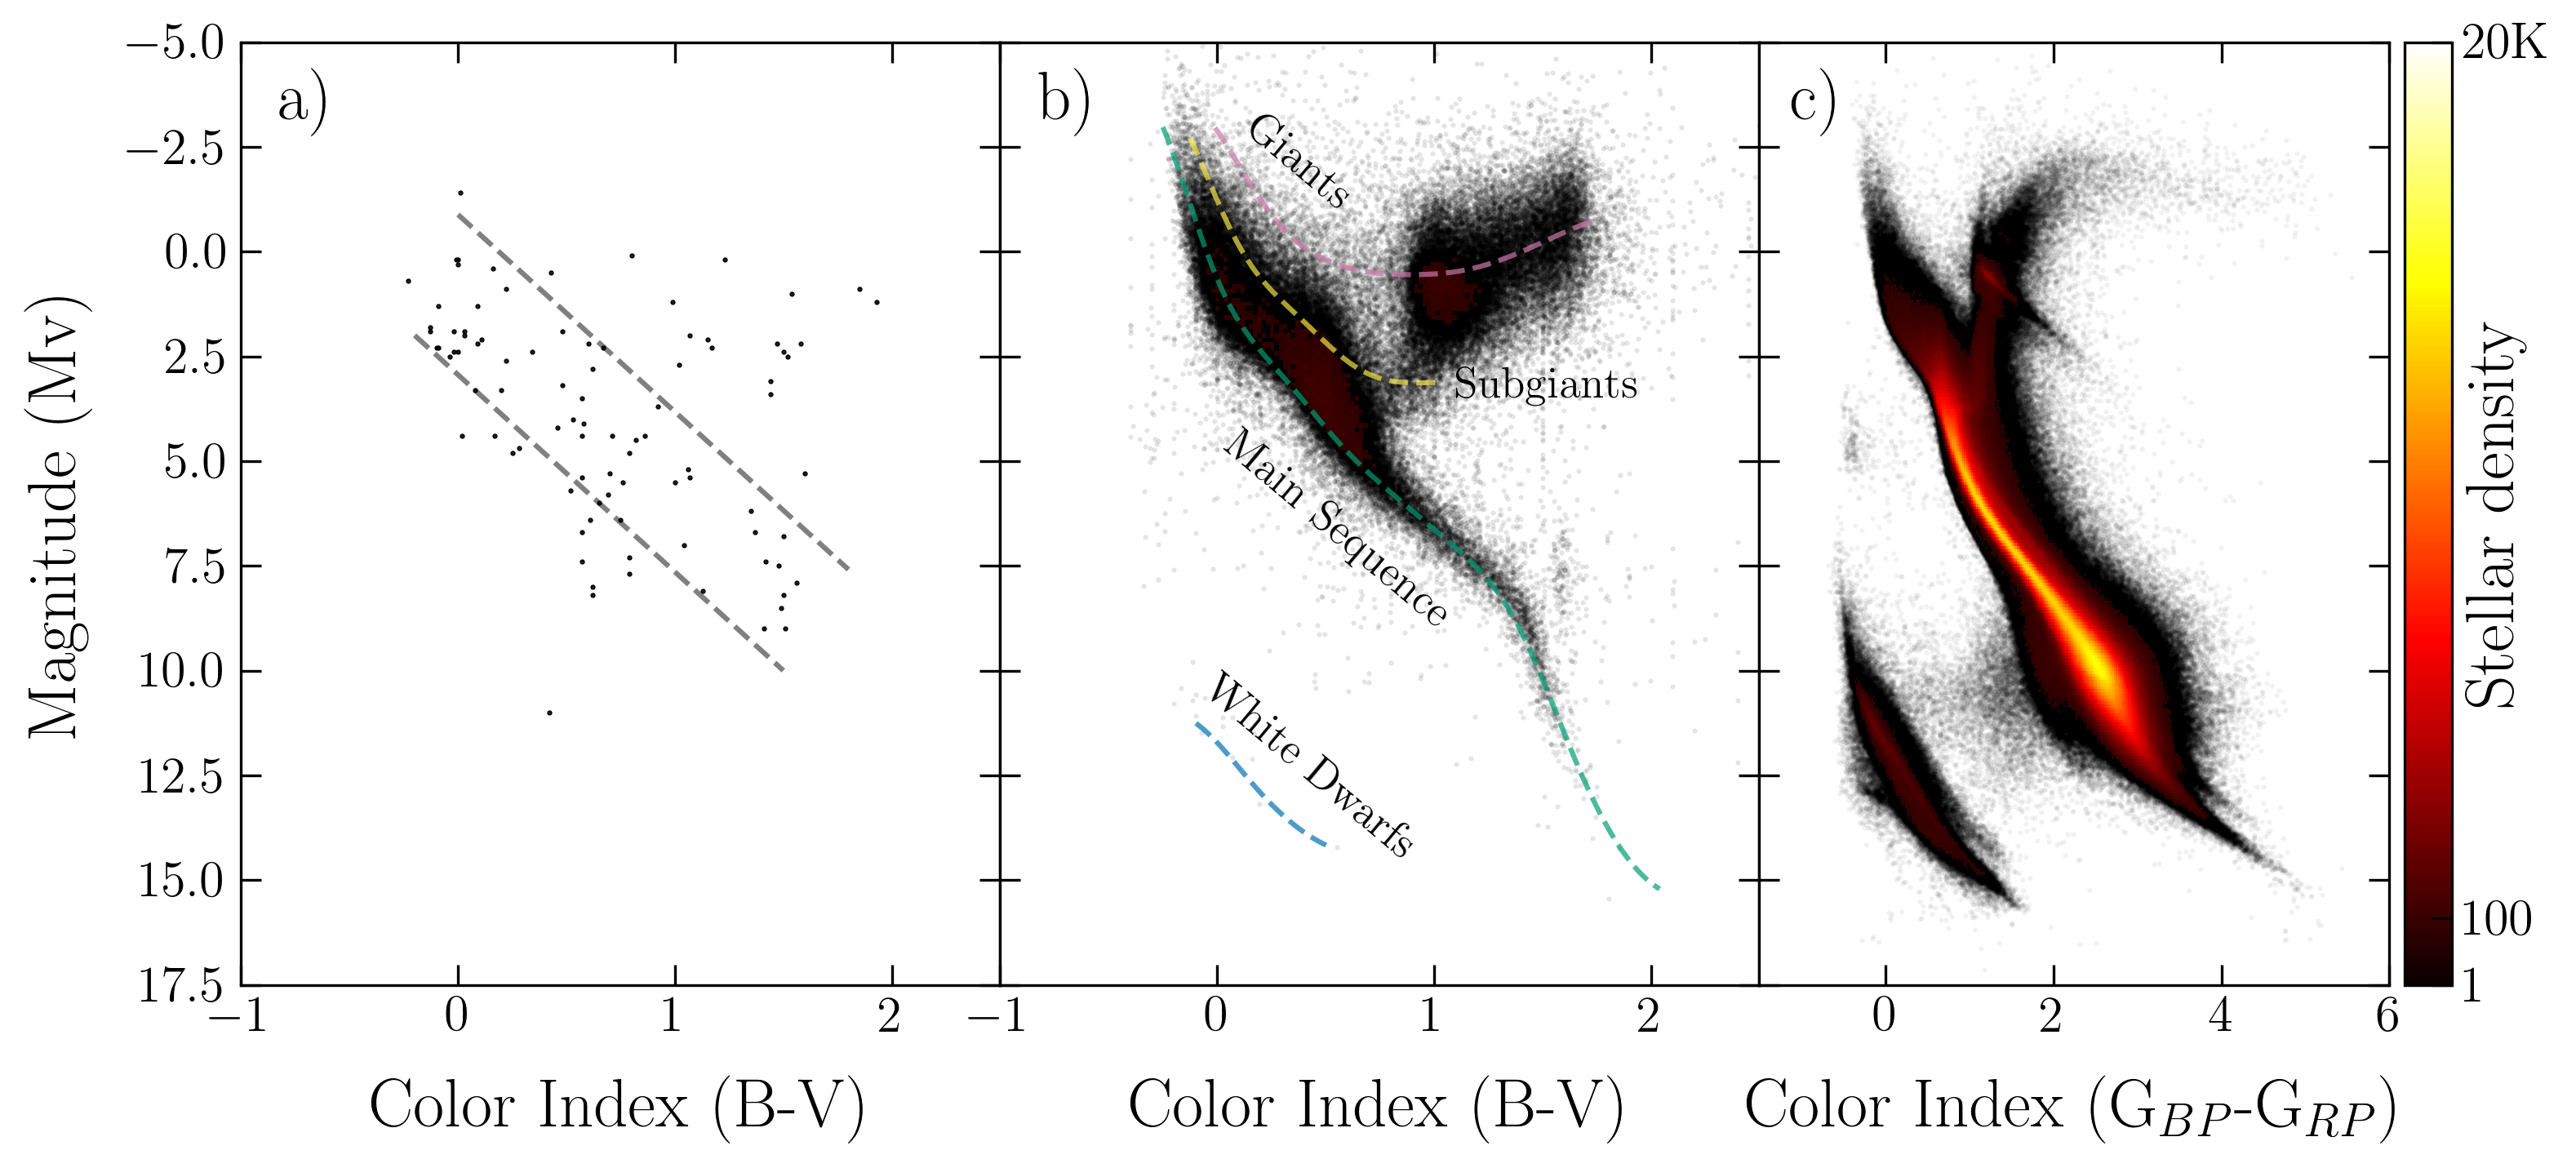
\includegraphics[width=1.2\linewidth]{figures/hr_diagram.png}}
  \caption{\textbf{Observational HR-Diagrams through the ages}: Catalog stars' color index is plotted on the horizontal axis and absolute magnitude on the vertical axis. Different regions of the diagram depend on the stars' masses, chemical composition, ages, and stages in the stellar life cycle. The color scale represents the number of stars in each portion of the diagram (black represents lower numbers of stars, and brighter colors correspond to increasingly higher numbers of stars). Panel (a) uses stars cataloged in 1914~\cite{Russell:1914:PA, 1914_HR_data}, panel (b) uses 1993 Hipparcos stars~\cite{HIPPARCOS}, and panel (c) uses 2022 Gaia stars~\cite{GaiaMission, GaiaEDR3}. Note: the 1914 stellar data was cross-referenced from the modern Hipparcos catalog to make this plot.
\github{https://github.com/avivajpeyi/hr_diagram_past_to_present}}
  \label{fig:HR-diagrams}
\end{center}
\end{figure}


The plot's data points helped Russell demonstrate that the temperature and luminosity of stars are related.
Brighter stars are displayed in the top part of the diagram, while dimmer stars are in the bottom. 
Bluer (hotter-surface) stars are on the left, and redder (cooler-surface) stars are on the right. 
Russell noted that most of the plotted stars fell in a band from the upper left to the lower right~\cite{Russell:1914:PA}.
He indicated this region with lines (the gray dashed lines reconstructed Figure~\ref{fig:HR-diagrams}a).
Russell and Hertzsprung also noticed a separate category of bright but cool red stars in the upper right corner~\cite{Russell:1914:PA, Hertzsprung:1911:POPot}.\footnote{Unfortunately, Hertzsprung's work was left unnoticed for a few years. Eddington chided Hertzsprung on this matter: ``One of the sins of your youth – to publish important papers in inaccessible
places''~\cite{Nielsen:1964:Cent}.}
They realised that these bright-cool red stars have a large surface area to produce high luminosity at low temperatures~\cite{Russell:1914:PA, Maury:1897:AnHar, Hertzsprung:1911:POPot}. 
Hertzsprung hence dubbed these as the ``giant" stars~\cite{Nielsen:1964:Cent}.  
Consequently, he named the less-luminous low-temperature red stars ``dwarf" stars. 
Russell recognised that the red dwarfs were just the bottom end of the band of stars within the gray lines in Figure~\ref{fig:HR-diagrams}a. 
Hence, Russell extended the grouping of ``dwarf" stars to the entire sequence, the sequence now known as the ``main sequence."
Even though the plot only contained a few stars, it provided Russell with a convenient way to illustrate his ideas about stellar evolution:
\myblockquote{The giant stars then represent successive stages in the heating up of a body and must be
more primitive the redder they are; the dwarf stars represent consecutive stages in later
cooling, and the reddest of these are the farthest advanced.}{Henry Russell, 1914}

Other astronomers like Eddington also used similar data and the HR diagram to drive some of their theories. 
For example, a decade later, Eddington's mass-luminosity relation would add evidence for stellar evolution down the main sequence~\cite{Eddington:1924:MNRAS}.
Soon, the HR diagram became a cornerstone diagram for modern astrophysics, and the concepts of stellar categories led to various advancements in our understanding of stellar physics~\cite{Nielsen:1964:Cent, 1914_HR_data}. 
Fortunately, since 1914, technological advances have created much larger samples of stars with well-measured properties, further improving our understanding of stellar physics.


\textbf{Jump to Hipparcos:}
Fast forward to seventy years in the future, the European Space Agency launched Hipparcos Satellite in 1989~\cite{HIPPARCOS}.\footnote{Hipparcos, an acronym for HIgh Precision PARallax COllecting Satellite, is also reference to Hipparchus, the ancient Greek astronomer who drew up the first accurate star map.}
One of the Hipparcos mission's primary goals was to provide a higher resolution observational HR diagram to obtain a detailed structure of stars with $M_v>0$ magnitude~\cite{HIPPARCOS}. 
In its four years of operation, this satellite cataloged nearly 120,000 stars~\cite{HIPPARCOS}. 
The Hipparcos catalog stars with low parallax errors, plotted in Figure~\ref{fig:HR-diagrams}b, show many more details than those in the 1914 HR diagram. 
Firstly, the vertical arm leading off the main sequence and turning to the right is much better defined -- this is the red giant branch indicating that as massive stars get older, they swell and become brighter and redder.
Similarly, the lower left of the diagram shows the white dwarf branch. 
The white dwarf region displays where the less massive stars (like our sun) that cannot undergo a supernova as they get older end up. 
Additionally, if we plotted stars with higher parallax errors, various other categories, such as the bright and super giants, are also visible.


\textbf{Gaia's gigantic data release:}
A few decades later, Hipparcos's successor Gaia made a considerable leap by cataloging 1.8 billion stars at an accuracy 200 times better than that of Hipparcos~\cite{GaiaMission, GaiaEDR3}. 
Figure~\ref{fig:HR-diagrams}c displays the Gaia stars with low parallax errors obtained in Gaia's third data release~\cite{GaiaEDR3}. 
This new HR diagram contains over 100 times more stars than Hippacros and allows astronomers to identify more refined details. 
For example, compare the hand full of white dwarfs in the Hipparcos diagram versus the thousands in the Gaia HR diagram.
This increase in white dwarf data has allowed astronomers to study the differences between white dwarfs made with helium cores and hydrogen cores~\cite{GaiaCollaboration:2018:AA}. 
Another exciting detail displayed in the Gaia HR diagram is the imprint of stellar binaries.
These binaries are present both in the main sequence and the white dwarf regions of the diagram (see the second tails at slightly higher magnitudes in both the main sequence and white dwarf regions of the plot).
The Gaia HR diagram appears to have a smaller red giant branch compared to Hipparcos's HR diagram~\cite{GaiaCollaboration:2018:AA}. 
However, the Gaia HR diagram has many more resolved features, such as the primary and secondary red clumps and the asymptotic giant branch bump. 
The sheer volume of the data made such discoveries possible. 
In addition to data on stellar temperatures and brightness, our catalogs now also contain stellar spectra and time-series data on stellar positions and proper motions~\cite{GaiaEDR3}.
This data has enabled astronomers to drive theoretical work and make inferences about the nature of stars.

This section demonstrates that novel observational data can spark major scientific breakthroughs, flashpoints of discovery. 
Each catalog of stars introduced here marks such a flashpoint. 
Each catalog's stellar data improved the calibration of stellar models, the study of stellar populations, and  overall comprehension of the cosmos. 
The following two sections of this chapter focus on two other areas where new astronomical data have created flashpoints. 

\section{The dawn of Gravitational wave astronomy}

%% What is a GW 
When some stars reach the end of their lives, they can turn into compact objects such as neutron stars and black holes. 
Some compact objects give away their positions via electromagnetic (EM) radiation due to accretion. 
Others reveal themselves via gravitational wave (GW) radiation emitted due to an oscillating mass quadrupole moment.
Any system with a gravitational quadrupole changing with time produces changes in its gravitational field, resulting in energy emission as gravitational waves.
Gravitational-wave astronomy gives us a new tool to examine the cosmos that complements classic electromagnetic astronomy.
Using gravitational waves, astronomers can research binary black holes and neutron stars that would otherwise be inaccessible.
However, it was only recently that astronomers were able to detect GWs. 

%% History of GW
In 1974, Russell Hulse and Joseph Taylor discovered a pulsar signal using the Arecibo radio telescope~\cite{Hulse:1975:ApJL}.
Measurements revealed that the pulsars' orbital period repeatedly fluctuates every few hours, indicating it is in orbit with a hidden companion.
Hulse and Taylor noted that the orbital period was decaying -- the pulsar and its companion were inspiralling~\cite{Hulse:1975:ApJL}.
After observing the system for another 30 years, they determined that the decrease of the orbital period resulted from the binary releasing gravitational waves, the first indirect observation of gravitational waves.

This indirect detection of gravitational waves paved the groundwork for the Laser Interferometer Gravitational-Wave Observatory, LIGO~\cite{Barish:1999:PhT}. 
LIGO was constructed in 1999, but it was not until 2015 that the first gravitational wave from a binary black hole merger, GW150914, was identified~\cite{abbott2016observation}.
Since then, the LIGO-VIRGO-KAGRA (LVK) collaboration has recorded several petabytes of data, and astronomers have discovered more than ninety gravitational wave signals from compact binary mergers~\cite{abbott2019gwtc, gwtc2, gwtc3}.
Individually, these events have provided astronomers with interesting information about various astrophysical objects. 
Taken together, the events form a population that can be studied as a whole. 

\begin{figure}
\begin{center}
  \centerline{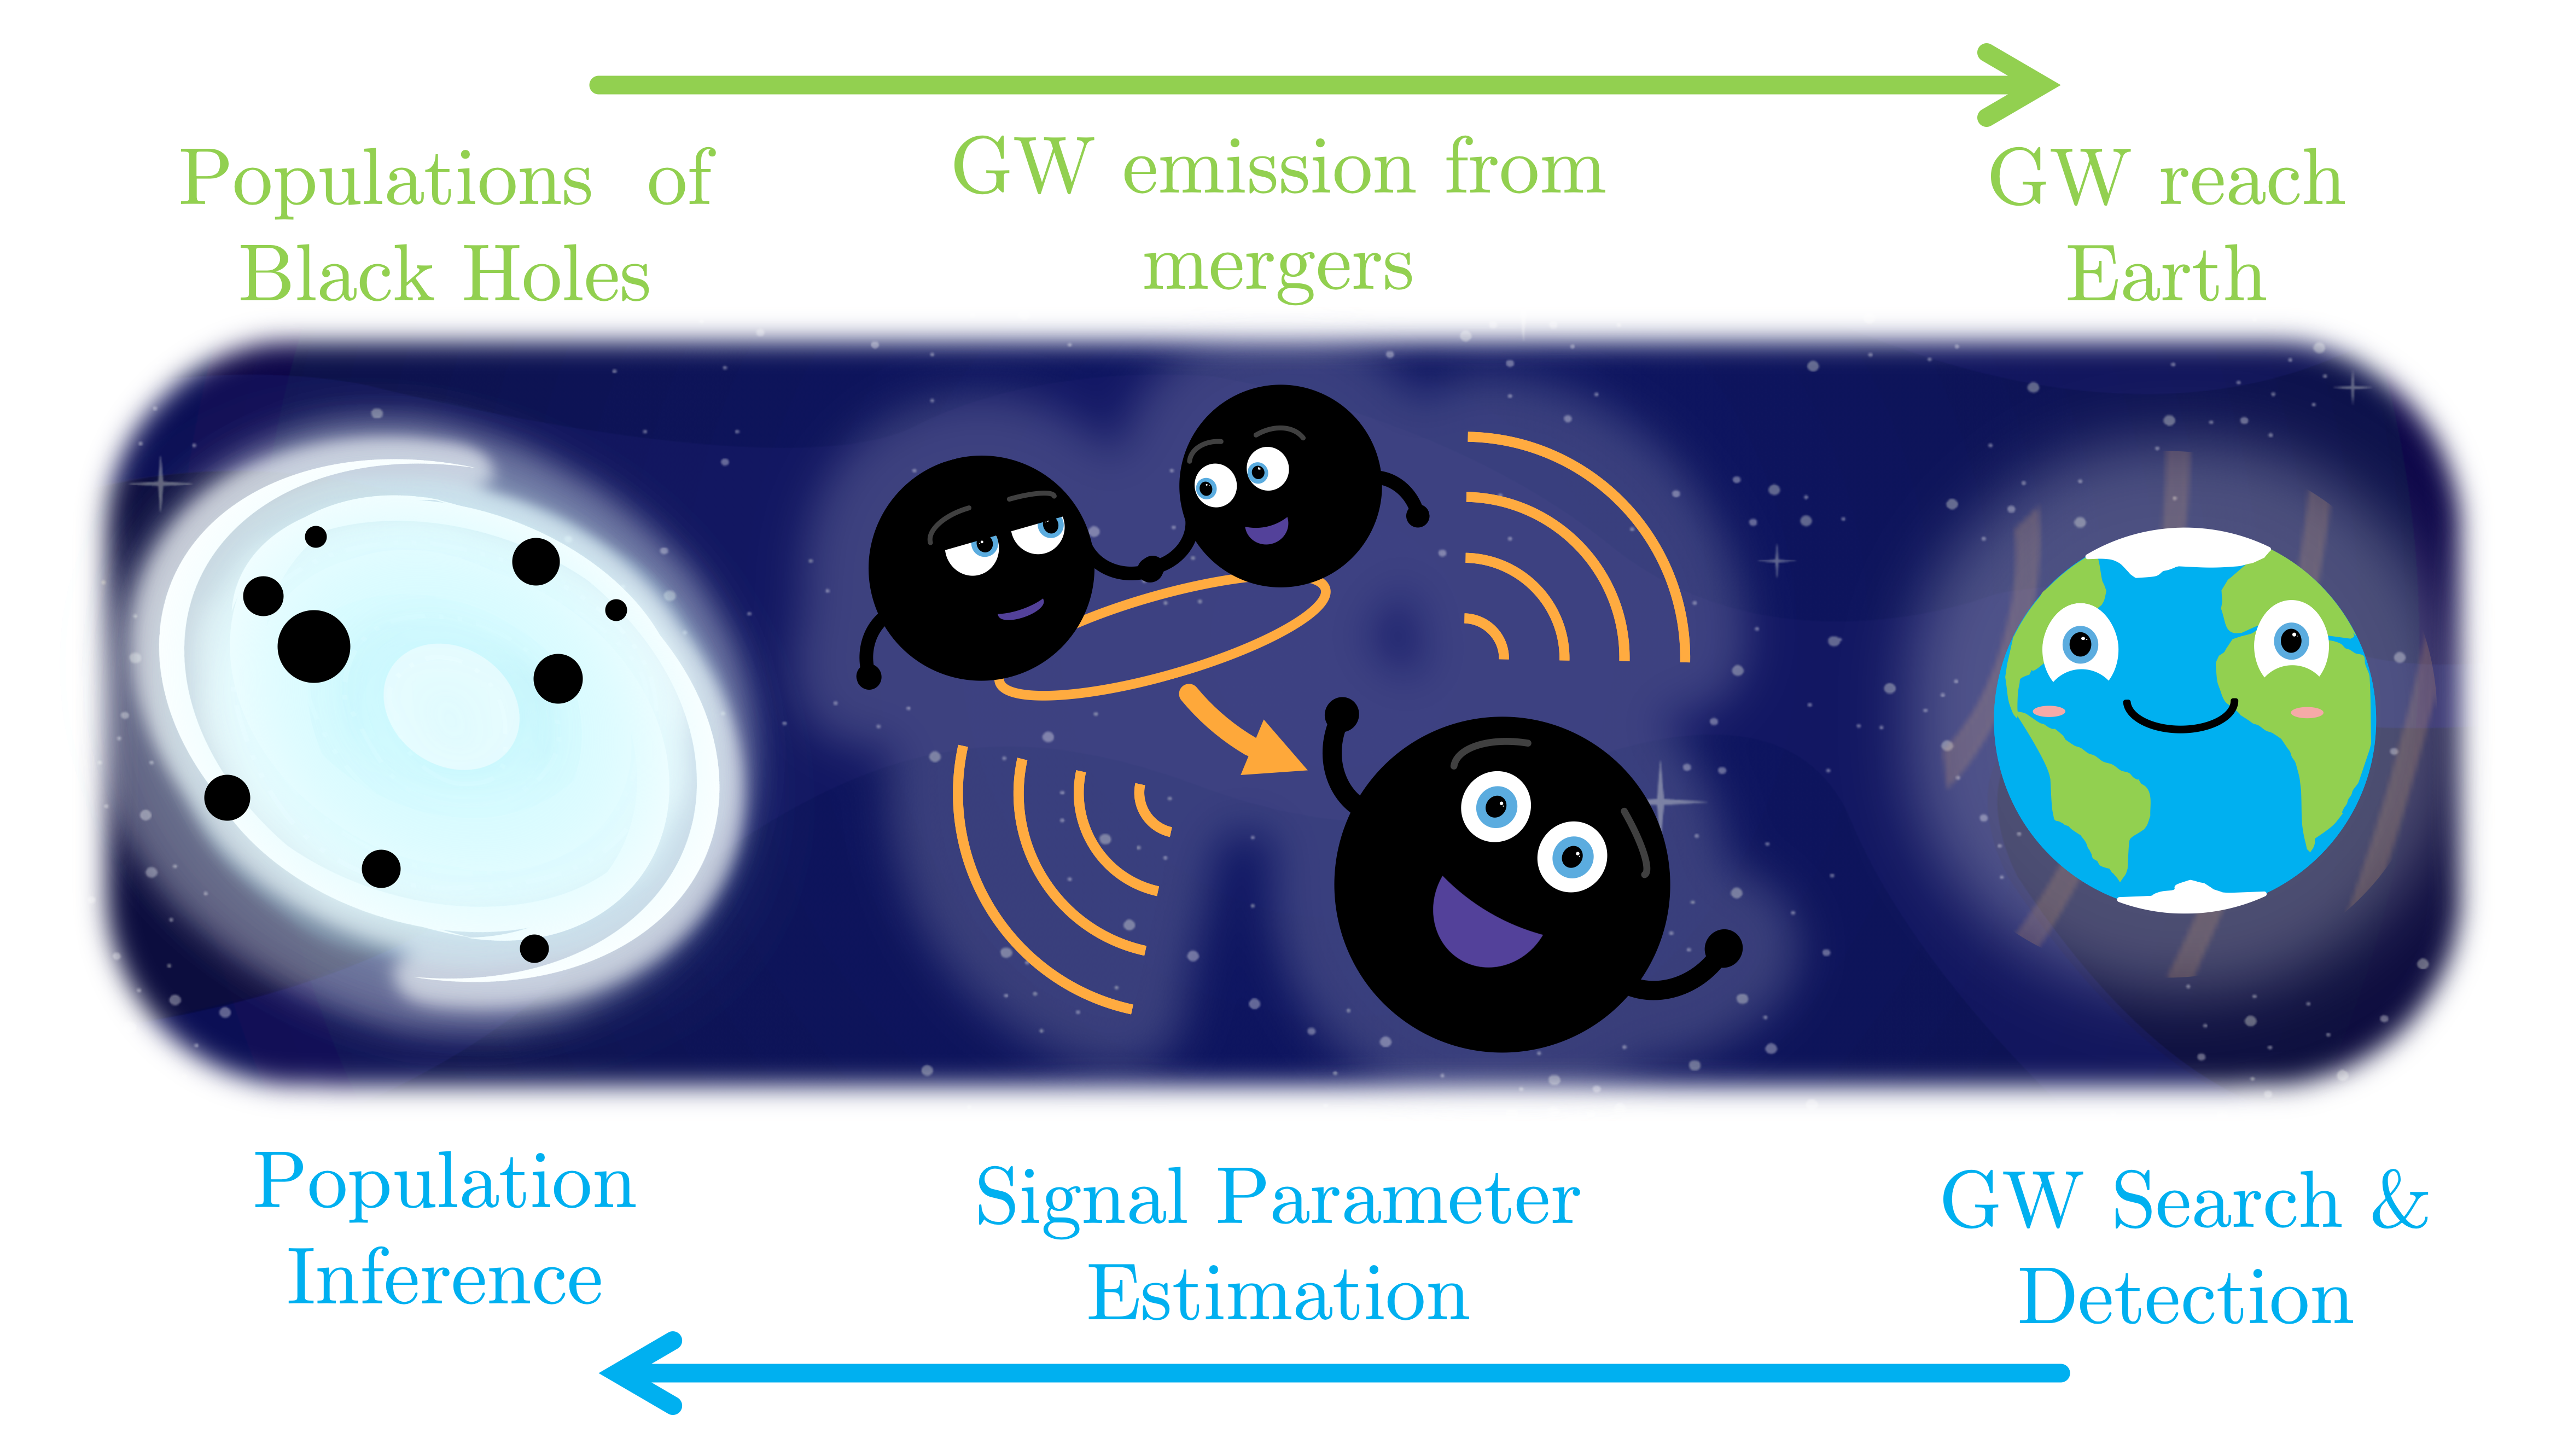
\includegraphics[width=1.1\linewidth]{src/figures/gw_pipeline.png}}
  \caption{\textbf{GW pipeline:} A schematic illustration of the steps taken in GW inference. \todo{Remove faces from this schematic}}
  \label{fig:gw_pipeline}
\end{center}
\end{figure}

The following sections introduce the LVK collaborations efforts to (i) search for GW signals from compact binary mergers, (ii) decode the GW signal parameters that describe the merger, and (iii) study the demographics of the merging black hole populations (each category and its goals are outlined in the schematic Figure~\ref{fig:gw_pipeline}).


\subsection{GW searches}  \label{sec:searches}

As LIGO records data, the data is immediately searched for generic, unmodeled  GW transients and modelled GW signals using low-latency search pipelines (there are also continuous and stochastic gravitational-wave searches, although they are not discussed here). 
These searches can identify candidate GW events in near real-time timescales, enabling the possibility of performing follow-up electromagnetic observations~\cite{abbott2018prospects, gw_search_review}.

The unmodeled gravitational-wave searches, like the Coherent Wave-Burst \textsc{cWB}~\cite{cWB_search} and Omicron-LIB \textsc{oLIB} piplines~\cite{oLIB} are performed without prior information about expected signal waveforms and instead involve cross-correlating the LIGO and Virgo detector data~\cite{gw_search_review}.
The cross-correlation is performed on the detector strain time series to look for excess power or bursts in the overlap region between the LIGO Hanford and LIGO Livingston detectors and between the LIGO Hanford and Virgo detectors, respectively \cite{gw_search_review}. 
Another unmodeled pipeline is \textsc{BayesWave}~\cite{Cornish:2015:CQGra}, which performs a \textit{follow-up} on the \textsc{cWB} candidates~\cite{bayeswave_as_followup, abbott2019all}. 
\textsc{BayesWave} fits the \textsc{cWB} candidates with both a GW signal model and an explicit glitch model (instrumental noise artefacts), both made up of sine-Gaussian wavelets and calculates the Bayesian evidence ratio, the Bayes factor, between the two competing hypotheses. 
The Bayes Factor is a measure of evidence for one model over another and can be used to compare models.
Such methods are effective at identifying GW transients that can last for
$10^{-3}-10^{1}$s~\cite{abbott2016observing}. 
Unmodeled gravitational-wave searches are powerful tools as they may help detect short-duration signals produced by unknown and known phenomena for which we have not yet developed good theoretical models~\cite{gw_search_review}. 
For example, short-duration signals from high mass binary black hole mergers, supernovae, cosmic strings, and unknown astrophysical phenomena as described in~\citep{abbott2018prospects}.

While unmodeled searches look for the unknown,  modelled or targeted gravitational-wave searches look for signals from known sources~\cite{abbott2016ligo}. 
Modeled searches for GW signals from the coalescence of compact binary coalescence (CBCs), such as \textsc{PyCBC}~\cite{biwer2019pycbc},
\textsc{GstLAL}~\cite{sachdev2019gstlal}, \textsc{MBTA}~\cite{MBTA} and \textsc{SPIIR} pipelines~\cite{SPIIR} use prior information about our expectations of GWs in searches~\cite{gw_search_review}. 
These searches compute the inner product between a gravitational waveform and the data stream and attempt to optimise the inner product by testing different waveforms. 
The different waveforms are chosen from a template bank of potential waveforms, where each waveform corresponds to different signal parameters. 

\begin{figure}
\begin{center}
  \centerline{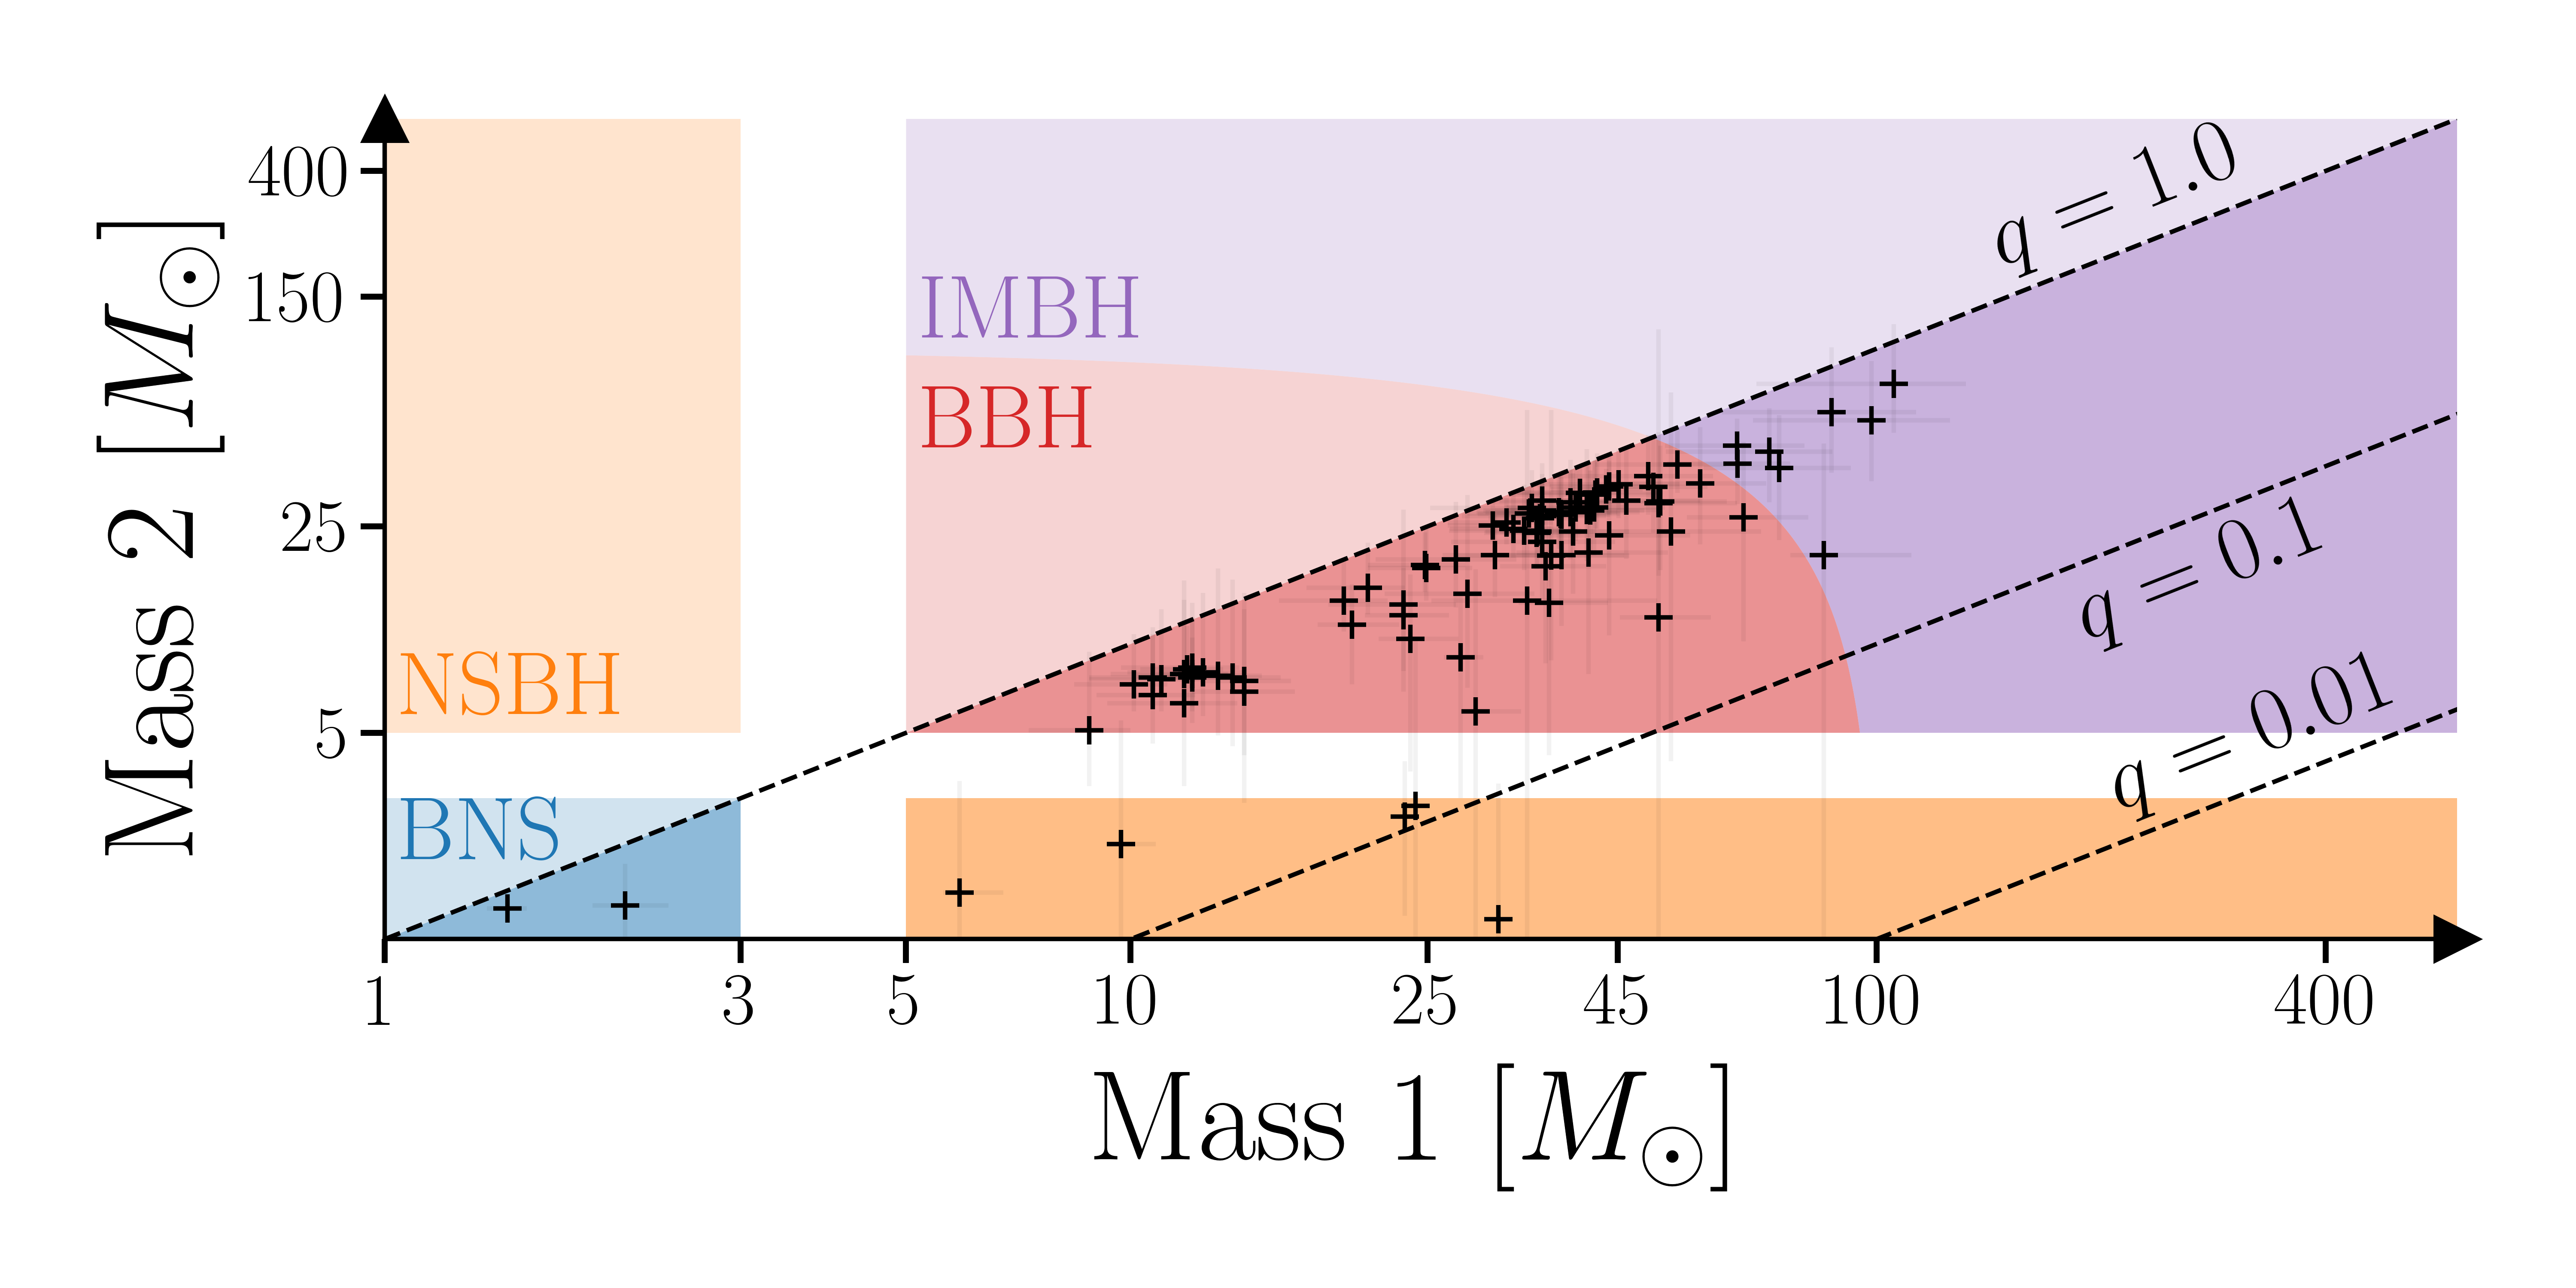
\includegraphics[width=1.1\linewidth]{src/figures/gw_catalog.png}}
  \caption{\textbf{CBC GW merger events:} Plot of the median (source frame) component masses of the CBC mergers in GWTC3~\cite{gwtc3}. The uncertainty bars are the 90\% credible interval values for each event. BNS, NSBH, BBH and IMBH stand for binary neutron star, neutron star -- black hole, binary black hole and intermediate-mass black hole mergers. \github{https://github.com/avivajpeyi/cbc_gw_catalog_plotter}}
  \label{fig:cbc_mergers}
\end{center}
\end{figure}

These search methods have successfully identified more than 90 CBC GWs, whose masses are plotted in Figure~\ref{fig:cbc_mergers}~\cite{gwtc3}.
If the detector data contained only gaussian noise and the occasional gravitational wave signal, these search pipelines would successfully identify all signals above some signal-to-noise ratio. 
Unfortunately, astronomers can also find glitches in the detector data~\cite{gw_search_review}. 
The search pipelines can mistake glitches for gravitational wave signals. 
Hence, the search pipelines also test signal coherence and compute `ranking statistics' to determine the statistical significance of candidates to prevent false positives. 

Efficient signal detection requires a ranking statistic that extracts the most information from the data to discriminate between noise and weak astrophysical signals~\cite{bci, bayeswave_as_followup, bcr_paper, bootstrap_gw, bcr_gw151216,bcr_gw151216, bayesian_odds}.  
However, existing CBC searches are sub-optimal: they do not provide a complete description of all features that may distinguish GWs from noise~\cite{bci}. 
Moving toward an optimal statistic (one that has a complete and accurate description of the signal and noise model) is a great challenge. 
Still, one way toward a better ranking statistic may be to demand that foreground triggers in two or more detectors should be better described as coherent gravitational-wave signals rather than incoherent glitches~\cite{bci}.
Importantly, it is not enough to provide some measure of coherence: one must also prove that an incoherent model is not more successful at describing the data. 

The Bayesian coherence ratio, \textsc{BCR}, proposed by \citet{bcr_paper} (based on \citet{bci}) can help take a step towards this optimal statistic~\cite{bci, bayeswave_as_followup, bcr_paper, bootstrap_gw, bcr_gw151216,bcr_gw151216, bayesian_odds}. 
As short-duration gravitational wave signals such as those from intermediate-mass black holes are the most challenging to distinguish from glitches, in Chaper~\ref{ch.bcr}, we investigate the usefulness of the \textsc{BCR} as a ranking statistic. 
Similar to how \textsc{BayesWave} can be used as a follow-up for \textsc{cWB} candidates, we demonstrate how the \textsc{BCR} can be used as a follow-up for \textsc{PyCBC} candidates. 

\subsection{GW Signal Parameter Estimation}

The core of parameter estimation in gravitational waves is Bayes' theorem. 
Given a model with parameters $\theta$, some data $d$ and the \textit{likelihood} $\mathcal{L}(d|\theta)$ of the data given the model, Bayes' theorem states that the \textit{posterior} $p(\theta|d)$ of model parameters given the data is 
\begin{equation}
{p(\theta|d)} = \frac{\mathcal{L}(d|\theta)\pi(\theta)}{\mathcal{Z}(d)}\ , \label{eq:bayeTheorem}
\end{equation}
where $\pi(\theta)$ is the \textit{prior} of the model parameters, and $\mathcal{Z}(d)$ is the marginalised likelihood known as the
\textit{evidence}. 
The evidence is the probability of the data itself, given the model:
\begin{equation}
Z(d) = \int_\theta \mathcal{L}(d|\theta)\pi(\theta)d\theta\ .
\label{eq:evid}
\end{equation}
As evidence is a probability of the data independent of model parameters, the evidences of two models on the same data help determine which model better describes the data.
Using gravitational wave models and equation~\ref{eq:bayeTheorem}, astronomers can compute the posterior probability of gravitational wave model parameters given some data containing a gravitational wave signal~\cite{abbott2018prospects}.
However, as CBC GW models can use more than 15 parameters to describe a signal, evaluating the posterior probability for gravitational waves is computationally expensive. 
For instance, consider analysing the posterior probability at ten grid points for each of the fifteen GW parameters.
This results in a massive number of points ($10^{15}$) for evaluating the posterior.
Additionally, far more grid points are required to accurately represent the continuous parameter space.
Moreover, because gravitational wave models incorporate sophisticated physics, their evaluation can be computationally expensive.
Altogether, evaluating the posterior over every point in parameter space represents an insurmountable computational obstacle.

An alternative way to estimate the posterior over a large parameter space is to utilise approaches such as Markov chain Monte Carlo (MCMC) and nested sampling to produce multivariate draws from the posterior~\cite{bilby_paper, bilby_gwtc, dynesty_paper, skilling2004, skilling2006}. 
These methods can also be parallelised to speed up the inference process. 
For a detailed discussion on the parallelisation of nested sampling and how it can boost gravitational-wave inference, refer to Chapter~\ref{ch.pbilby}. 


\subsection{Interpretting GW signals}

After GW searches and parameter estimation pipelines identify and characterise signals, astronomers can begin interpreting the inferred parameters.
Mass and spin inferences help determine where (e.g., isolated space, globular clusters, or active galaxies) these binaries form and merge.
Each observation's inferred parameter can reveal the binary's formation pathway.


For example, consider the inferred parameters for GW150914, GW190521 and GW190425~\cite{abbott2016observation, gw190521,gw190425}. 
The observation of GW150914 robustly demonstrates that relatively ``heavy'' black holes ($\geq25\ M_{\odot}$) can form and eventually even merge~\cite{gw150914_asto_implications}.
Based on GW150914's component black hole masses, astronomers inferred the stellar progenitors may have existed in a low-mass galaxy in the local Universe~\cite{gw150914_asto_implications}. 
GW190521's parameters show that the signal originated from an asymmetric BBH merger with masses of $85^{+21}_{-14}M_{\odot}$ and $66^{+17}_{-18}M_{\odot}$~\cite{gw190521}.
The remnant object was the first direct detection of an IMBH with a mass surpassing the pulsational-pair instability mass gap.
Due to its large initial masses, some believe this may be a second-generation merger and hence is improbable to be a field merger. 
On the other hand,  parameter estimation of GW190425 suggests the event's binary had a non-circular orbit, indicating it may have come from a globular cluster~\cite{Romero-Shaw:2020:MNRAS}.

Similarly, the community has recently been discussing GW151226~\cite{Chia:2022:PhRvD, Mateu-Lucena:2021:arXiv, Nitz:2021:ApJ}. 
Initial research concluded that GW151226 resulted from a CBC with conventional masses and spins, as seen in Figure~\ref{fig:gw151226_cases} (case A), and hence was likely a field-binary.
However, recent work by \citet{Chia:2022:PhRvD} suggests that the GW emerged from a peculiar system: an asymmetric BBH merger with misaligned  spins (case B). Such a configuration would unlikely exist in the field~\cite{Chia:2022:PhRvD}.

%% GW151226 Figure
\begin{figure}
\begin{center}
  \centerline{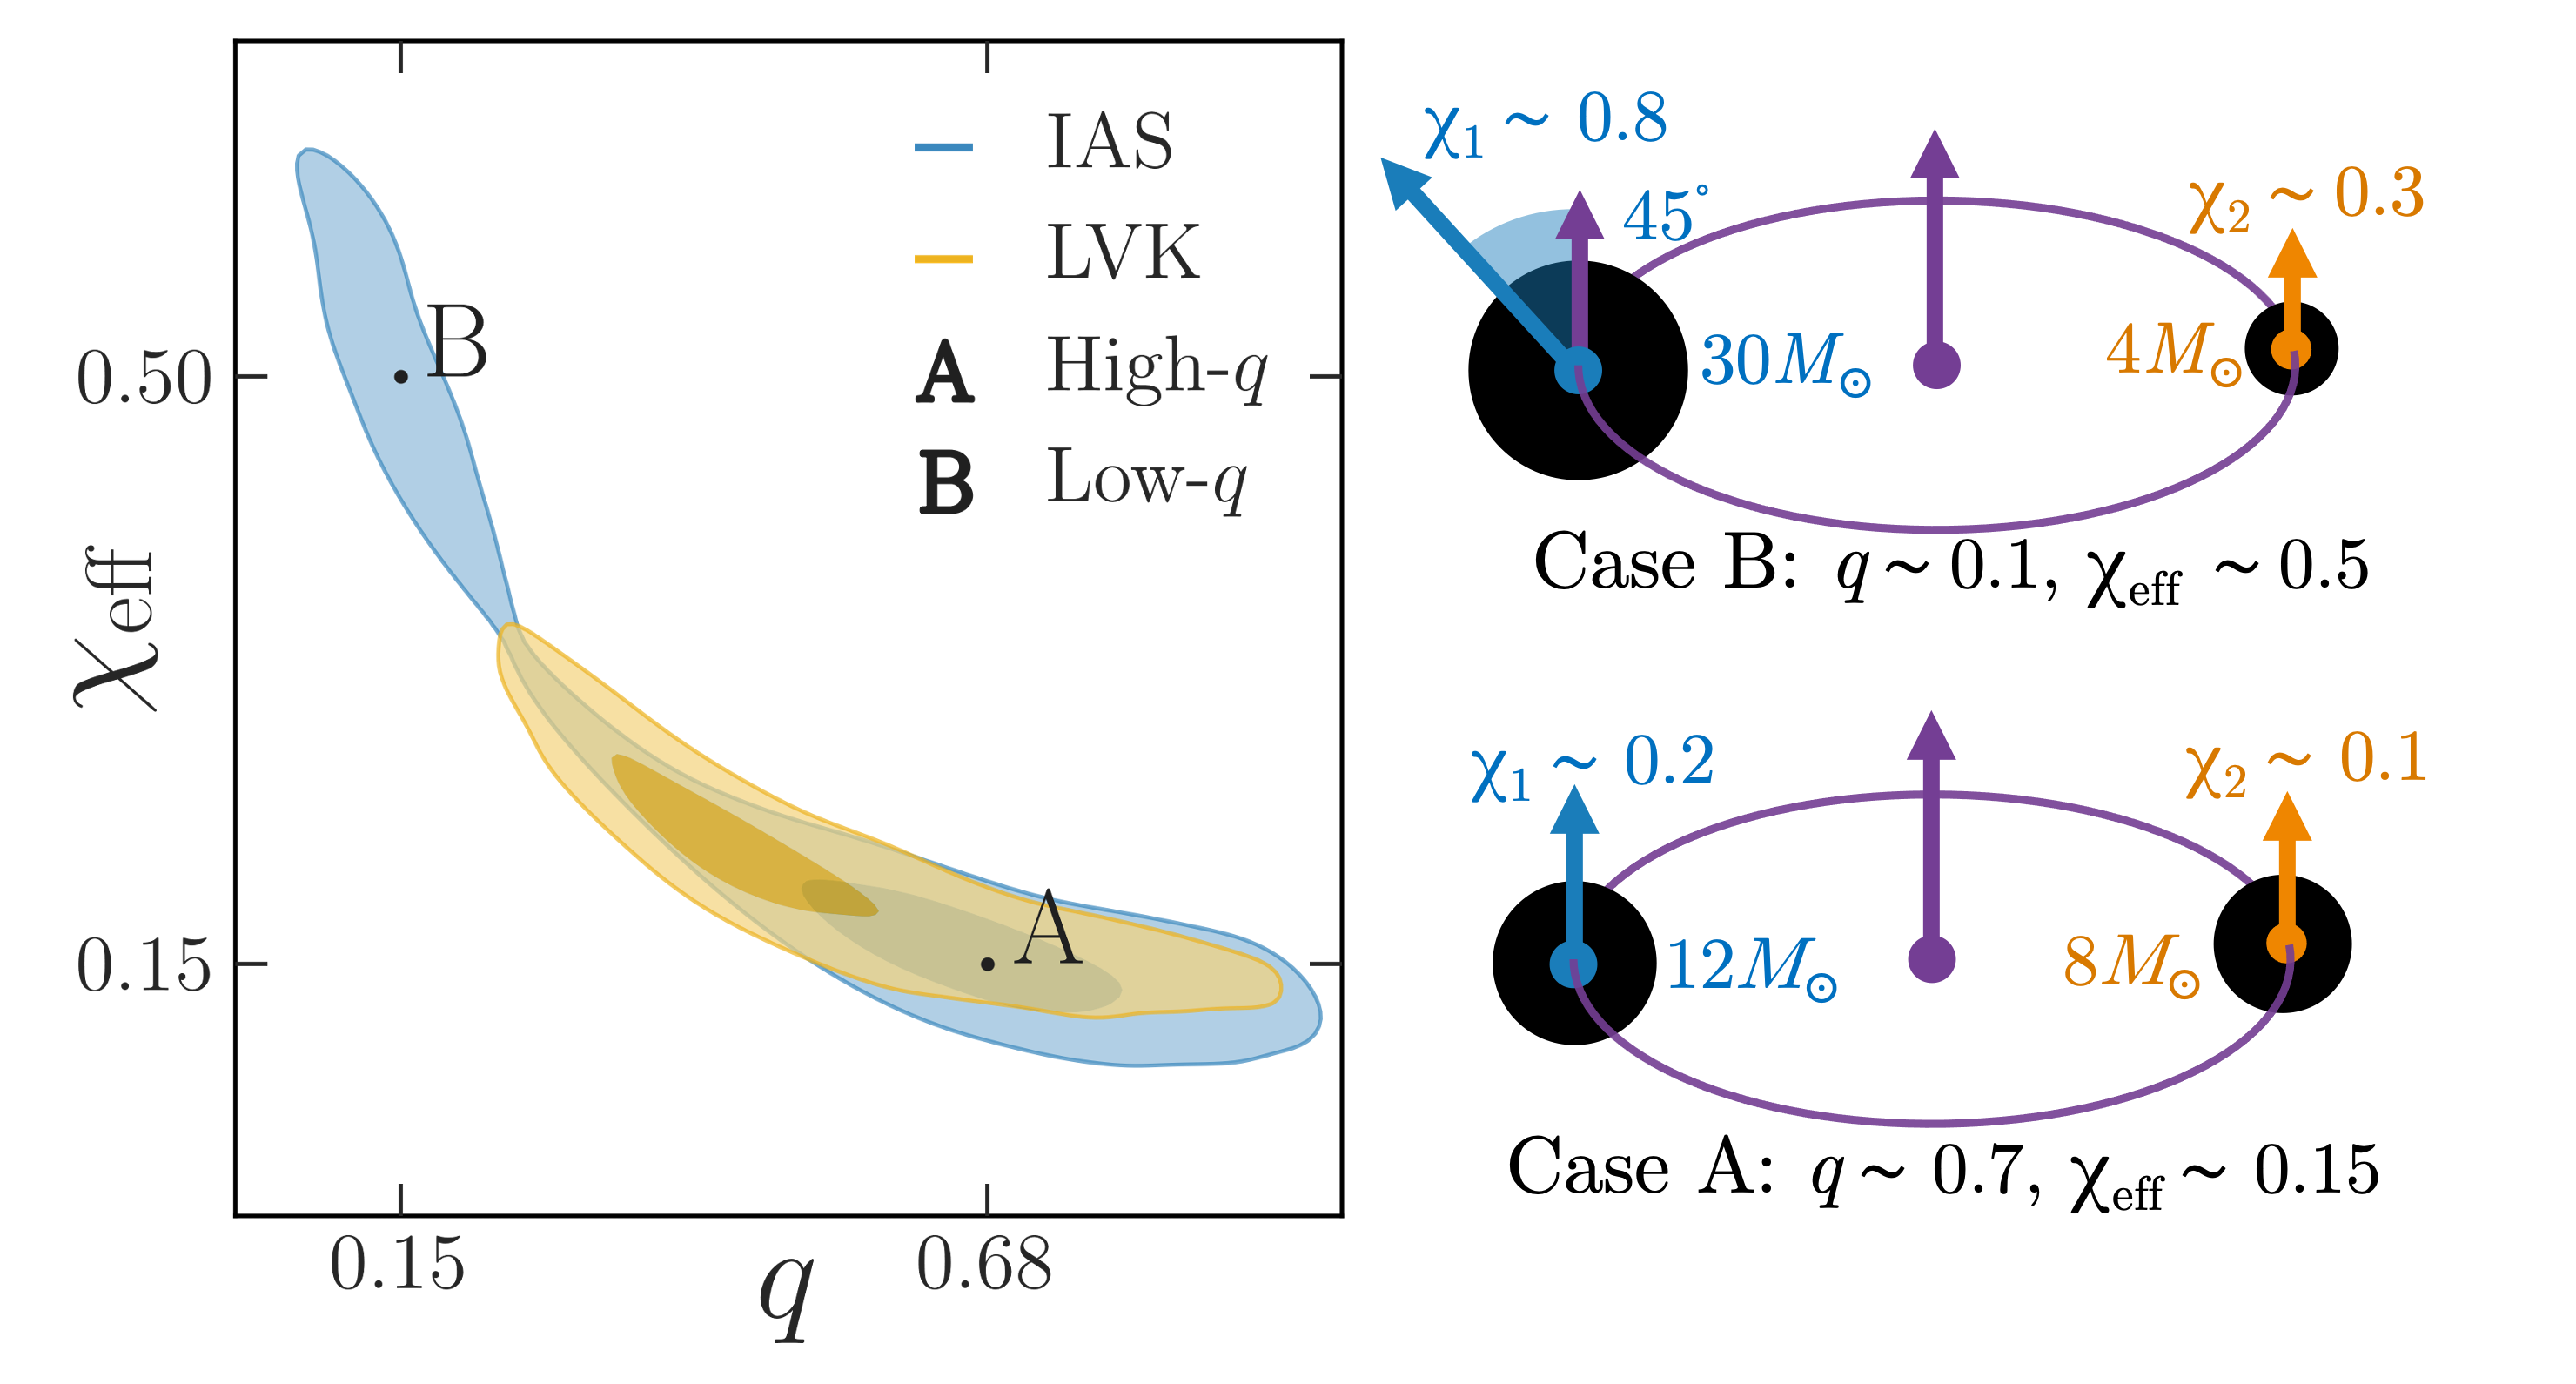
\includegraphics[width=1.1\linewidth]{src/figures/gw151226_cases.png}}
  \caption{\textbf{GW151226 Cases:} The left side displays $q-\chi_{\rm eff}$ posteriors from the \citet{Chia:2022:PhRvD} analysis (labeled the IAS posterior) and \citet{Mateu-Lucena:2021:arXiv}'s analysis (labeled the LVK posterior as it used the same configuration as the LVK analysis). The right side displays a schematic illustration of the two BBH cases. \todo{Change Case a and Case B to point A and point b (to avoid people thinking of Case A/B mass transfer)}
  }
  \label{fig:gw151226_cases}
\end{center}
\end{figure}


It is uncertain which of these cases is most likely, making it difficult to establish this event's formation channel.
Chapter~\ref{ch.deep} presents a ``deep follow-up'' tool to determine which case is  more probable.
It employs Bayesian model selection to evaluate the posterior odds of two points by computing the points' marginal likelihood.
The posterior odds for case A versus B are near 1, reflecting that it is valid to interpret GW151226's binary to have been from either case.

\subsection{GW population inference}

With many GW events, astronomers can also study the ensemble properties of merging systems, such as how masses and spins of all detected BHs are distributed, using hierarchical inference techniques~\cite{gwtc12population, gwtc3population}.
The LVK has used several hypotheses in hierarchical inference studies to map ensemble mass and spin distribution features to astrophysical processes  described by stellar evolution and population synthesis models.
For example, recent work on the black hole spin population has examined computing the fraction of signals expected to result from isolated-field binary mergers versus dynamical binary mergers.
In Chapter~\ref{ch.agn}, we look into another binary merger channel: the active galactic nuclei (AGN) channel.
AGNs are promising environments for the assembly of merging binary black hole systems with large masses (e.g. GW190521~\cite{mckernan2020black}), asymmetric masses (e.g. GW190425~\cite{mckernan2022ligo}), and a variety of spin configurations~\cite{tagawa2020spin, Ford:2021:arXiv, mckernan2020monte}. 

\begin{figure}
\begin{center}
  \centerline{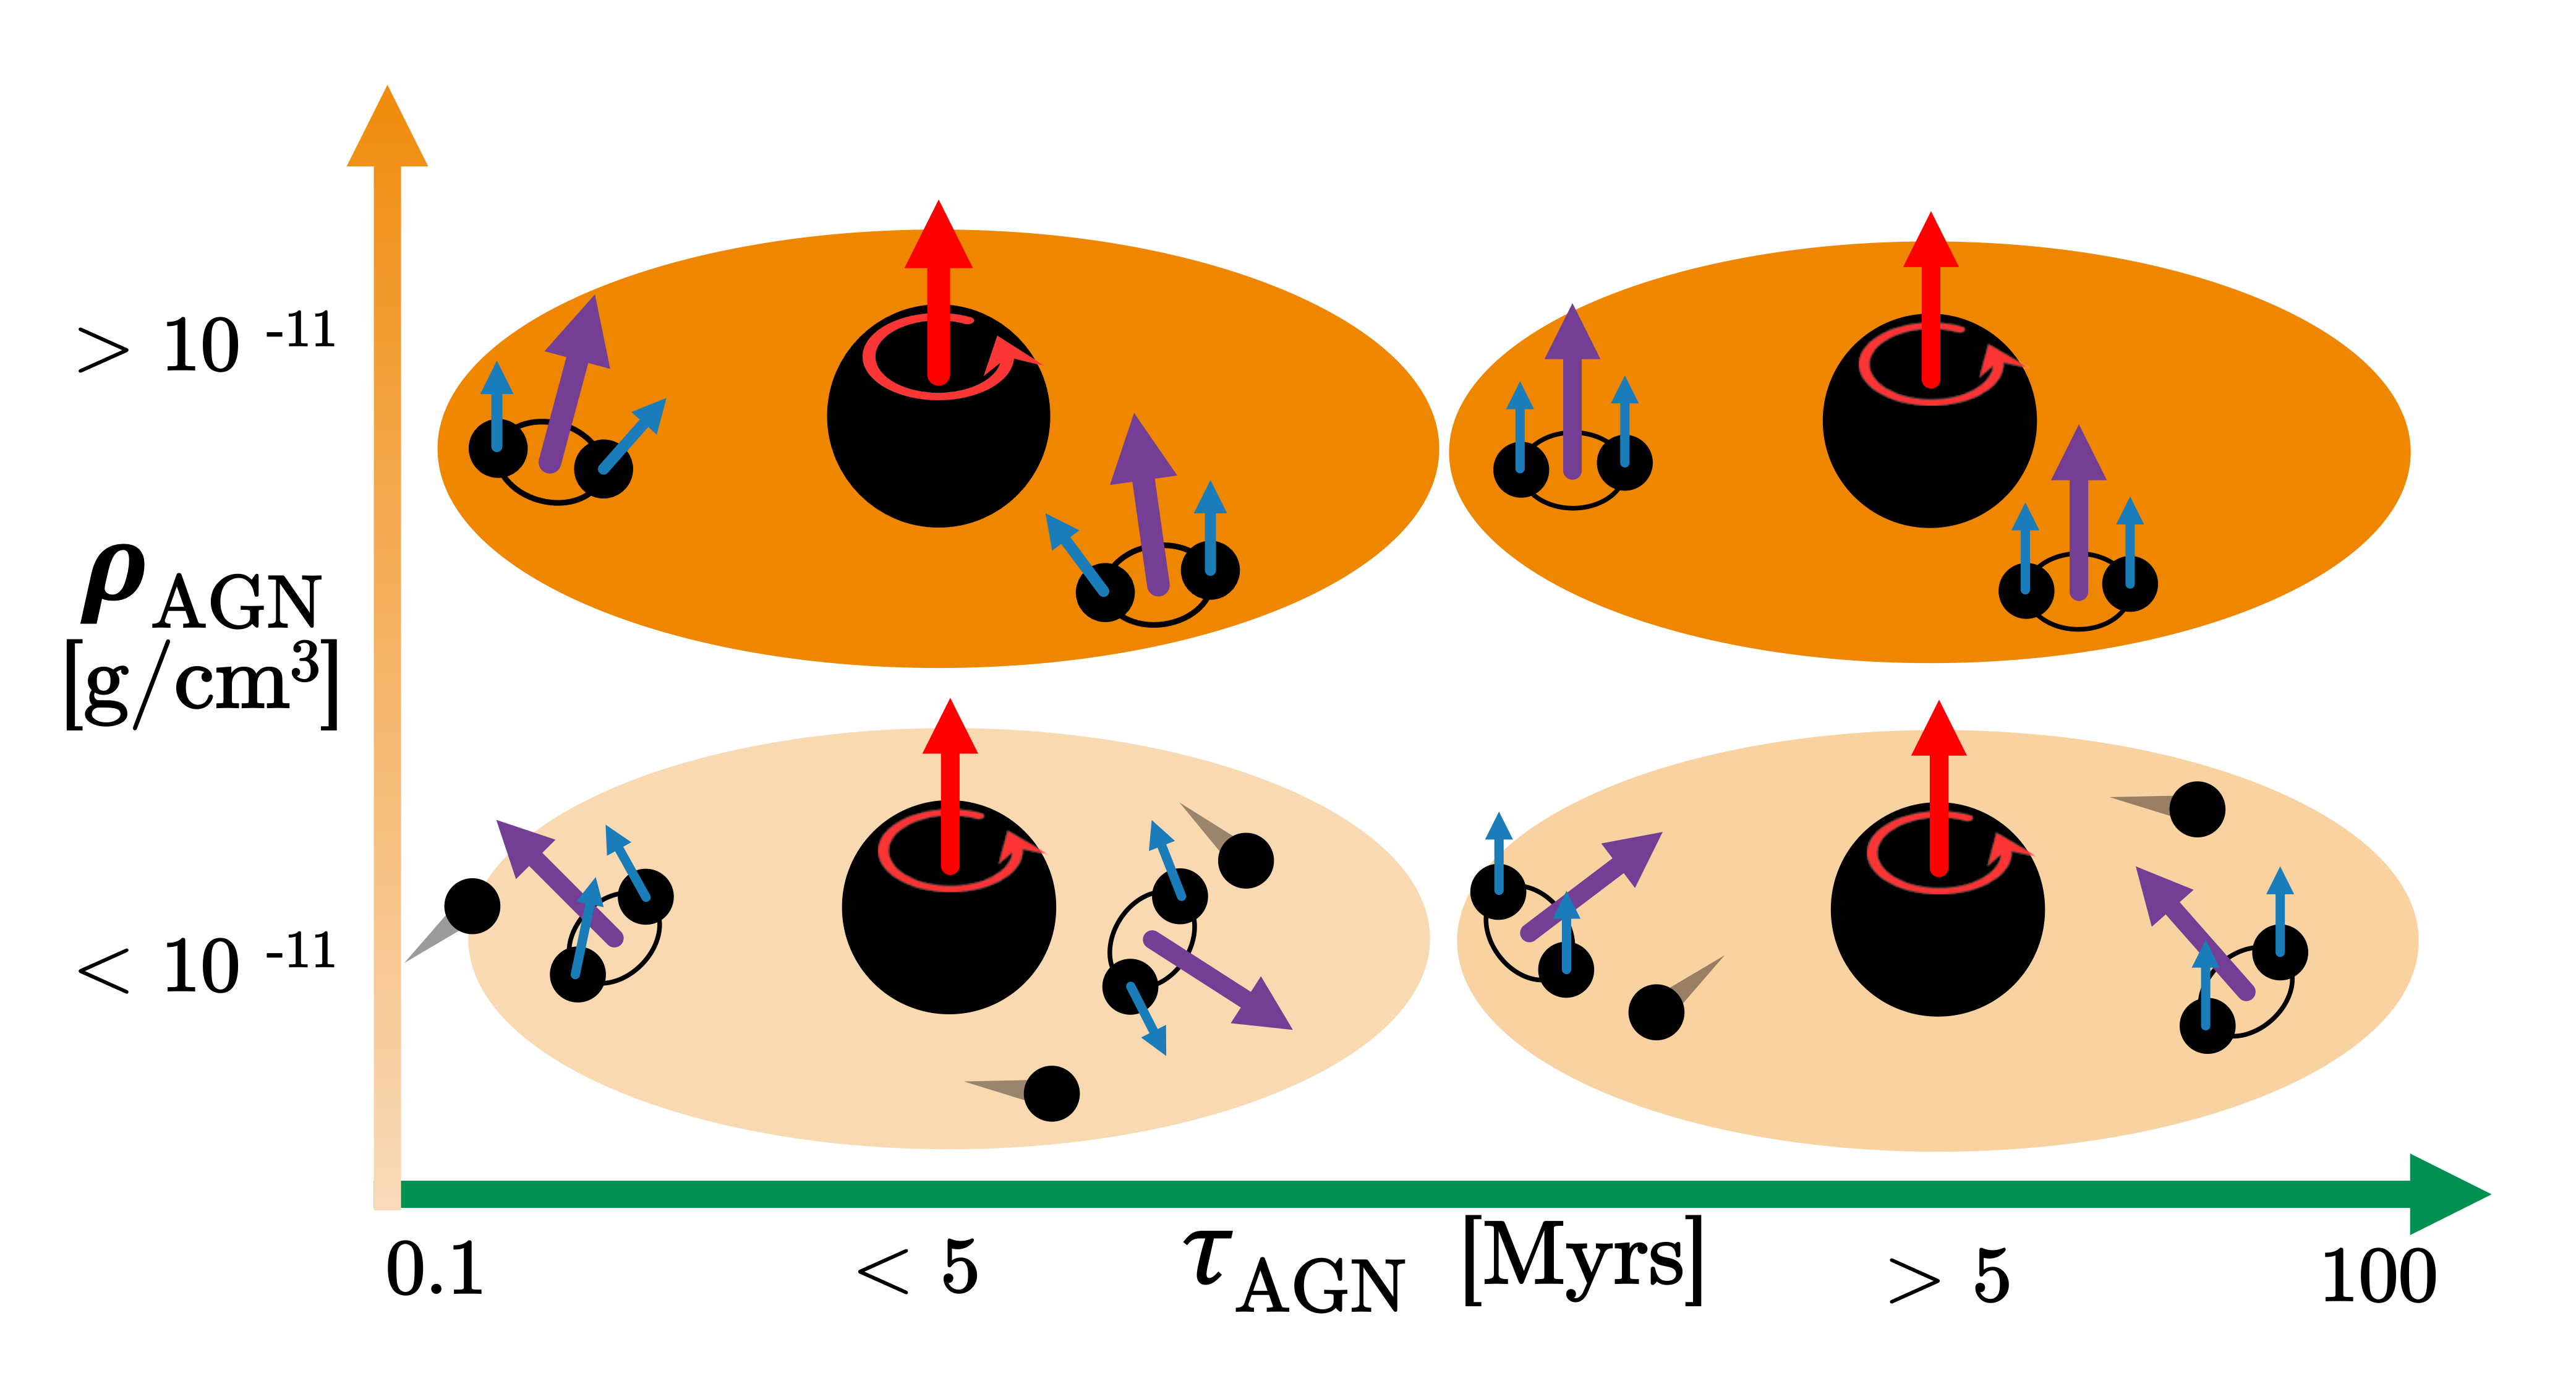
\includegraphics[width=1.\linewidth]{src/figures/agn_spins.png}}
  \caption{\textbf{AGN BBH-spins:} Different AGN age $\tau_{\rm AGN}$ and density $\rho_{\rm AGN}$ values can lead to different binary black hole spins. The different scenarios are described in the text.}
  \label{fig:agn_spins}
\end{center}
\end{figure}


In Chapter~\ref{ch.agn} we draw on simulations of BBH systems in AGN to propose a phenomenological model for the distribution of black hole spins of merging binaries in AGN disks~\cite{agn_migration_trap, agn_bbh_rates, agn_orbital_evol, agn_migration_1, agn_migration_2}. 
The model incorporates distinct features that make the AGN channel potentially distinguishable from other channels, such as assembly in the field and globular clusters. 
The model parameters can be mapped to the age $\tau_{\rm AGN}$ and density $\rho_{\rm AGN}$ of AGN disks. 
A schematic illustration of the model is presented in Figure~\ref{fig:agn_spins}. 
In the Figure's top right corner, where the AGN is old and dense, the BBH orbital angular momentum and component BH spins align with the central SMBH spin. 
Conversely, all spins are misaligned in the lower left, where the AGN is young and dilute. The other two corners represent unique spin orientations described in further detail in Chapter~\ref{ch.agn}.
In Chapter~\ref{ch.agn} we demonstrate how these different populations of binaries in AGNs can be distinguished.
If most merging black holes are assembled in AGNs, future gravitational-wave observations may provide insights into the dynamics of AGN disks.

\section{The hunt for exoplanets}

Humans have long sought worlds beyond our own to answer questions like: how did the planets in our solar system form? Are Earth-like planets common? And, the biggest question of all -- is there life beyond Earth? 
The answer to the last question will change humankind forever, whether it reveals a universe replete with rare and fragile life, or no life. 
Nevertheless, just as our ability to locate faraway stars or detect gravitational waves was constrained by technology until relatively recently, so was our ability to investigate planets beyond our solar system, exoplanets.
Now, thanks to the Kepler and TESS satellites, astronomers have found thousands of exoplanets.
Although no traces of life have been identified, scientists have learned that these worlds vary greatly in size and temperature and are composed of the same elements as the planets in our solar system~\cite{Traub:2012:ApJ, Morris:2017:ApJ, Yu:2017:ApJ}.
This section reviews the hunt for exoplanets, and some of what we have learned from the exoplanets found so far.

\subsection{Planets beyond the solar system: search and discovery}
Sometimes, serendipity plays a role in science.
The first  exoplanet observation is one such incident.
As the world trembled from the onset of World War I in 1917, Walter Adams was recording the spectrum of a white dwarf star on a glass plate.
The spectrum of this star contains unusually heavy components, such as magnesium and iron~\cite{Farihi:2016:NewAR}.
These contaminants could not have evolved naturally within the star. 
Thus they must have originated from the shattered remains of an exoplanet.
Unfortunately, Adams was unaware of this, and his finding stayed in the archives until 2016 when Jay Farihi discovered and correctly interpreted Adam's work~\cite{Farihi:2016:NewAR}.

Since Adams' observations, many scientists have reported discoveries of exoplanet candidates.
Unfortunately, all candidates were disproven until 1992 when Aleksander Wolszczan and Dale Frail published their work on a bizarre system~\cite{wolszczan1992planetary}. 
Wolszczan and Frail were investigating  pulsar PSR B1257+12's periodic timing variations.
After extensive investigation, they concluded the periodicity was due to two planets orbiting the pulsar. 
Astronomers were initially surprised by this planetary system because they anticipated that supernovae that generated pulsars would kill or eject any planets in orbit via a shockwave. 
Therefore, the scientists hypothesised that these two planets may have formed when the destroyed planets' gas and dust accumulated around the pulsar after the supernova~\cite{wolszczan1992planetary}.
Exciting as it was, Wolszczan and Frail's exoplanet was not what scientists were seeking; the hunt for the first exoplanet orbiting a sun-like star continued.
Only three years later, the hunt resulted in the discovery of exoplanet ``51Pegasi b'' by Didier Queloz, a doctoral student, in 1995~\cite{mayor1995jupiter}.
Queloz discovered this massive exoplanet with an orbit of 4 days using the ``radial-velocity'' method, in which the slight wobble of a star is measured due to the gravitational pull of an orbiting planet. 


\begin{figure}
\begin{center}
  \centerline{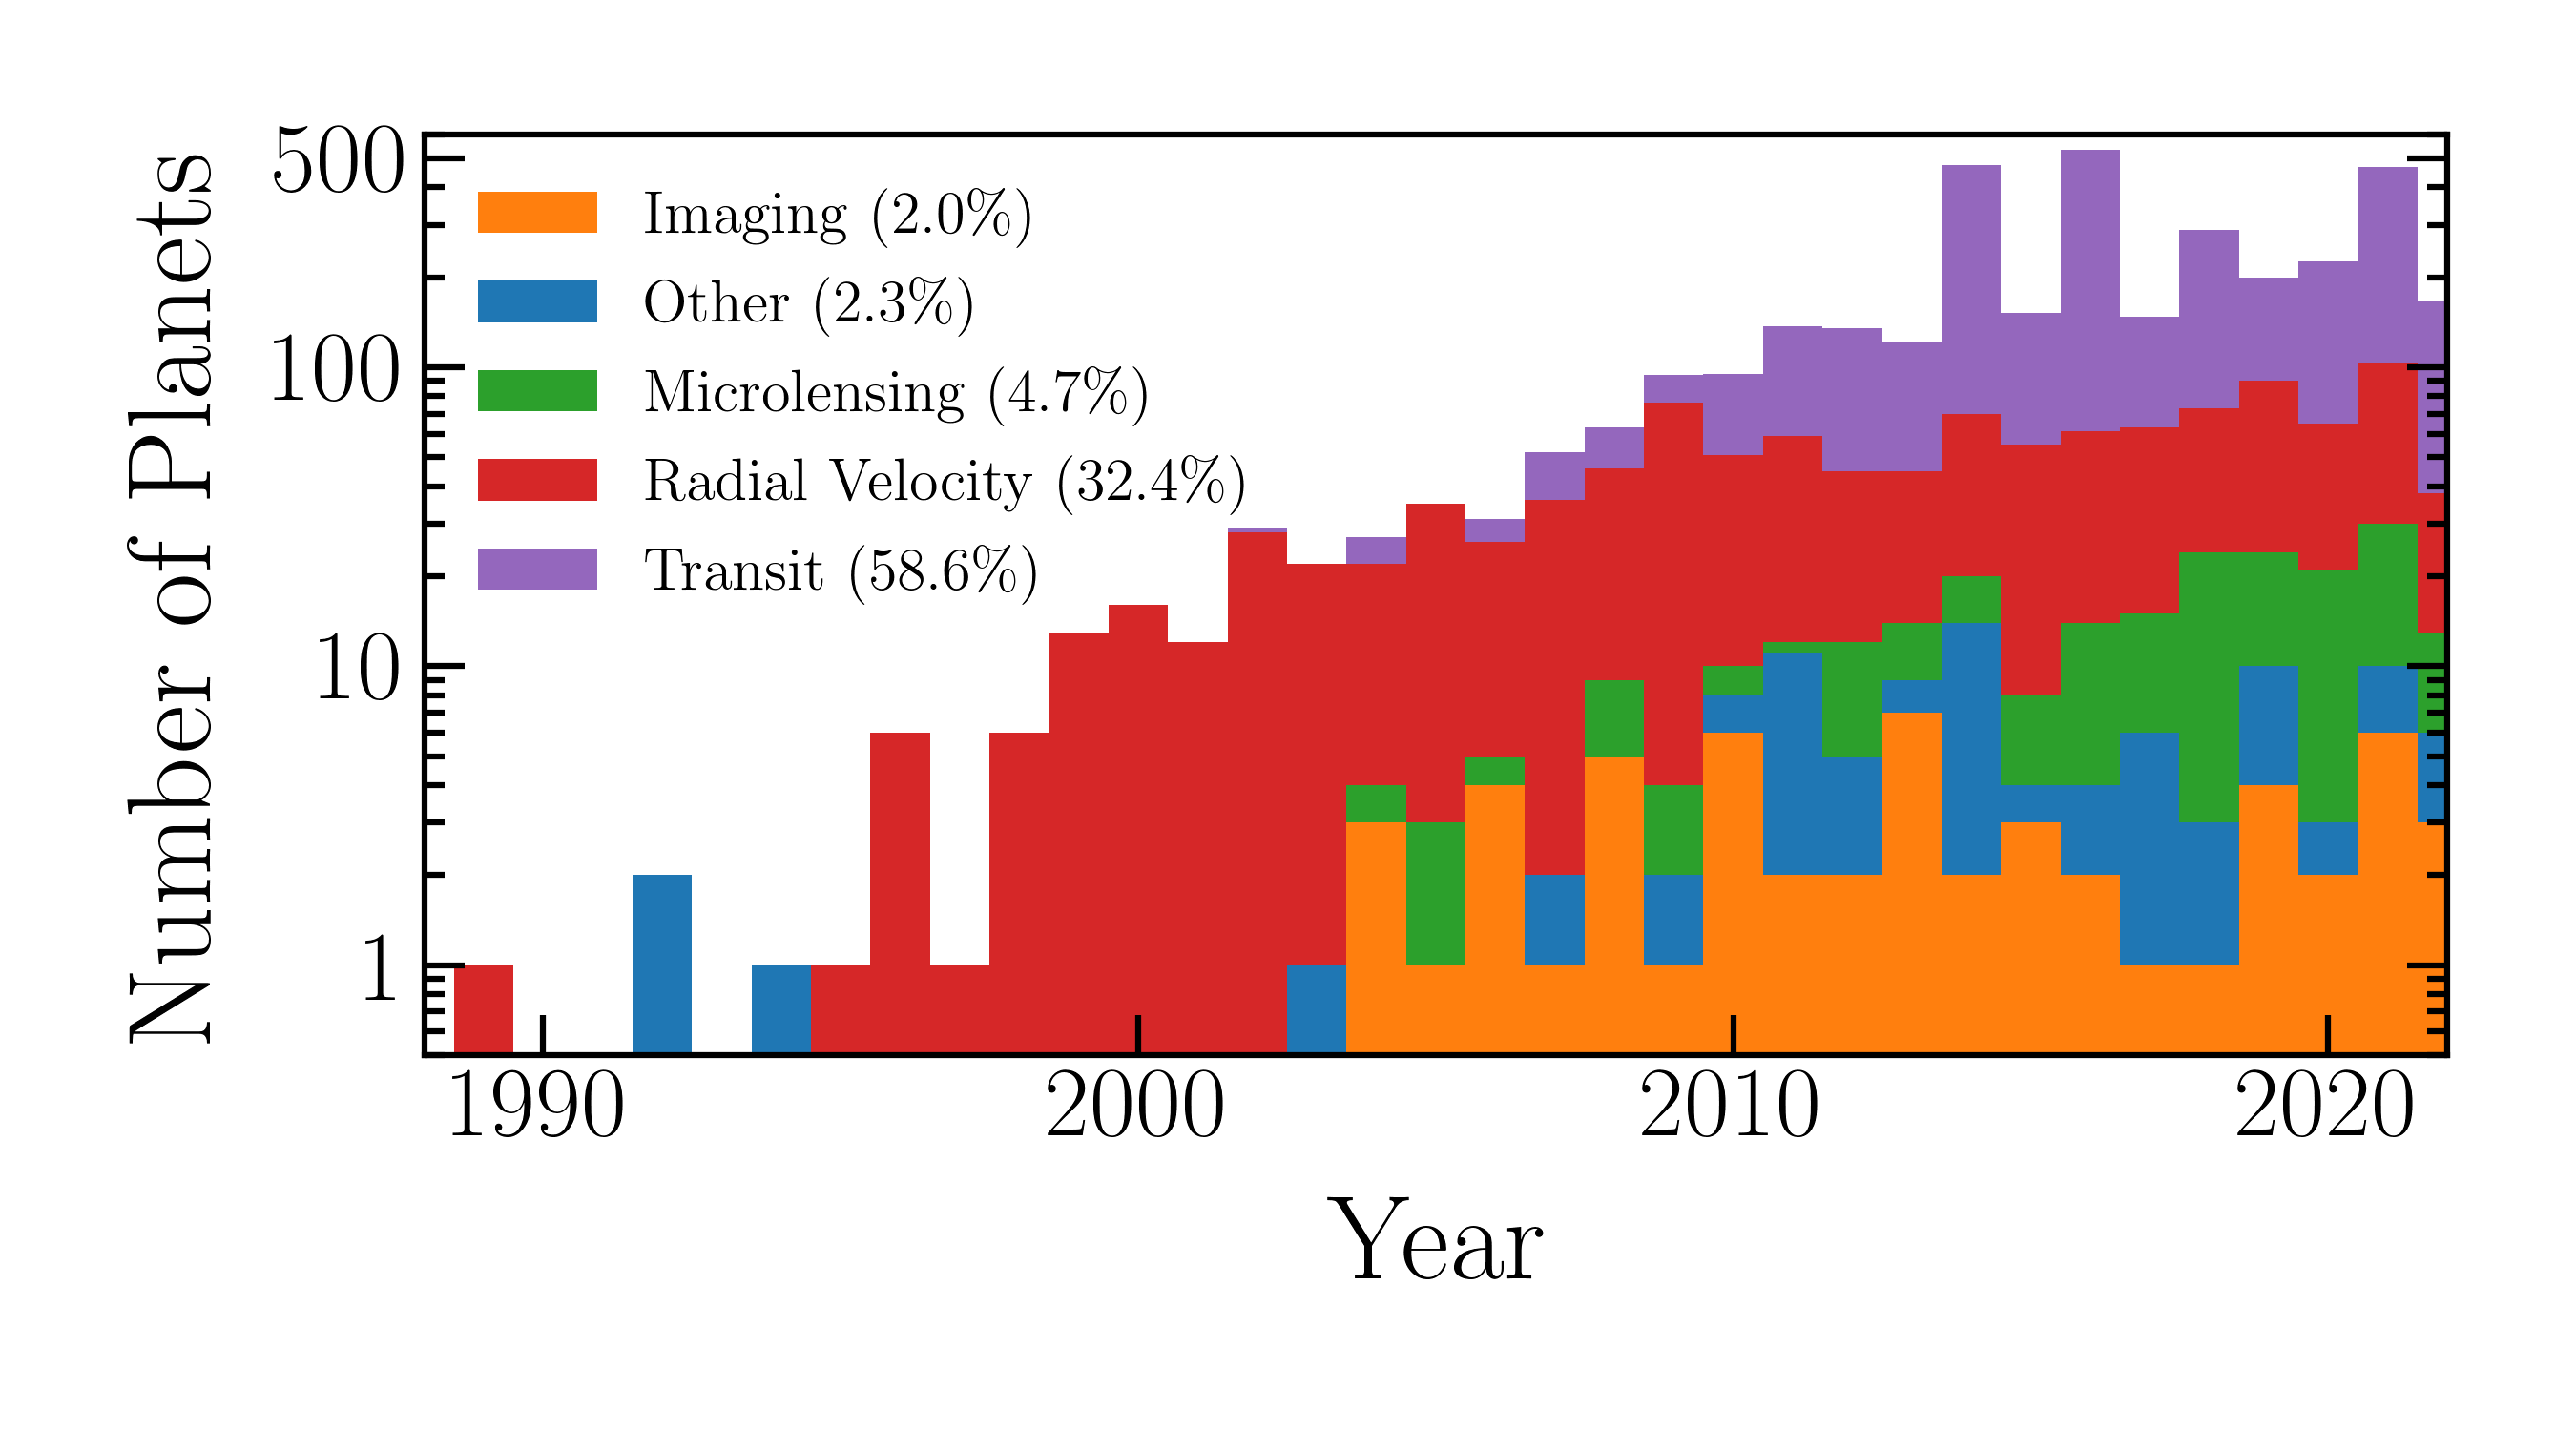
\includegraphics[width=1.\linewidth]{src/figures/confirmed_planets_vs_time.png}}
  \caption{\textbf{Exoplanet detections over time:} A cumulative bar plot showing the number of exoplanets discovered per year. The top panel is colored by the telescope used for detections. The bottom panel is colored by the method used to identify the exoplanet. Data has been obtained from \href{https://exoplanetarchive.ipac.caltech.edu/}{\textsc{ExoFop}}. \github{https://github.com/avivajpeyi/exoplanet_catalog_plotter}}
  \label{fig:exo_detections_over_time}
\end{center}
\end{figure}


Several other exoplanets with radial velocity were discovered after 1995.
In 1999, \citet{charbonneau1999detection} utilised a network of three 10-cm telescopes\footnote{Some of these telescopes were set up in parking lots~\cite{david_exoplanet_parkinglot}!} to focus on the star of a recently discovered exoplanet.
They identified the exoplanet using the transit method, which looks for periodic dips in a star's brightness caused by an orbiting planet blocking some light~\cite{charbonneau1999detection}.
Soon, the transit method became the most effective technique for discovering exoplanets.

Figure~\ref{fig:exo_detections_over_time} plots the number of exoplanet discoveries from 1989 to 2022. 
The graphic illustrates that the transit approach has discovered the most extrasolar planets, followed by the radial velocity method.
The data also indicate that the number of exoplanet discoveries has increased significantly over time.
Launches of the Kepler and TESS satellites helped to boost the number of detections.

Launched in 2009, Kepler observed 530,000 stars in the Cygnus constellation and confirmed over 2,600 exoplanets. 
Before its retirement in 2018, analysis of Kepler's data established that there are more planets than stars in our galaxy~\cite{Swift_2013} with 20-50\% of stars having small (potentially Earth-like) planets~\cite{Fressin:2012:Natur, Petigura:2013:PNAS}, and that there appear to be different categories of planets~\cite{Traub:2012:ApJ, Morris:2017:ApJ, Yu:2017:ApJ}.
Finally, Kepler data showed that the Solar System was the most peculiar planetary system discovered to date~\cite{Weiss:2018:AJ}. 
The following sections delve into some of these discoveries.

\subsection{From Hot Jupiters to Habitable Super-Earths}


\begin{figure}
\begin{center}
  \centerline{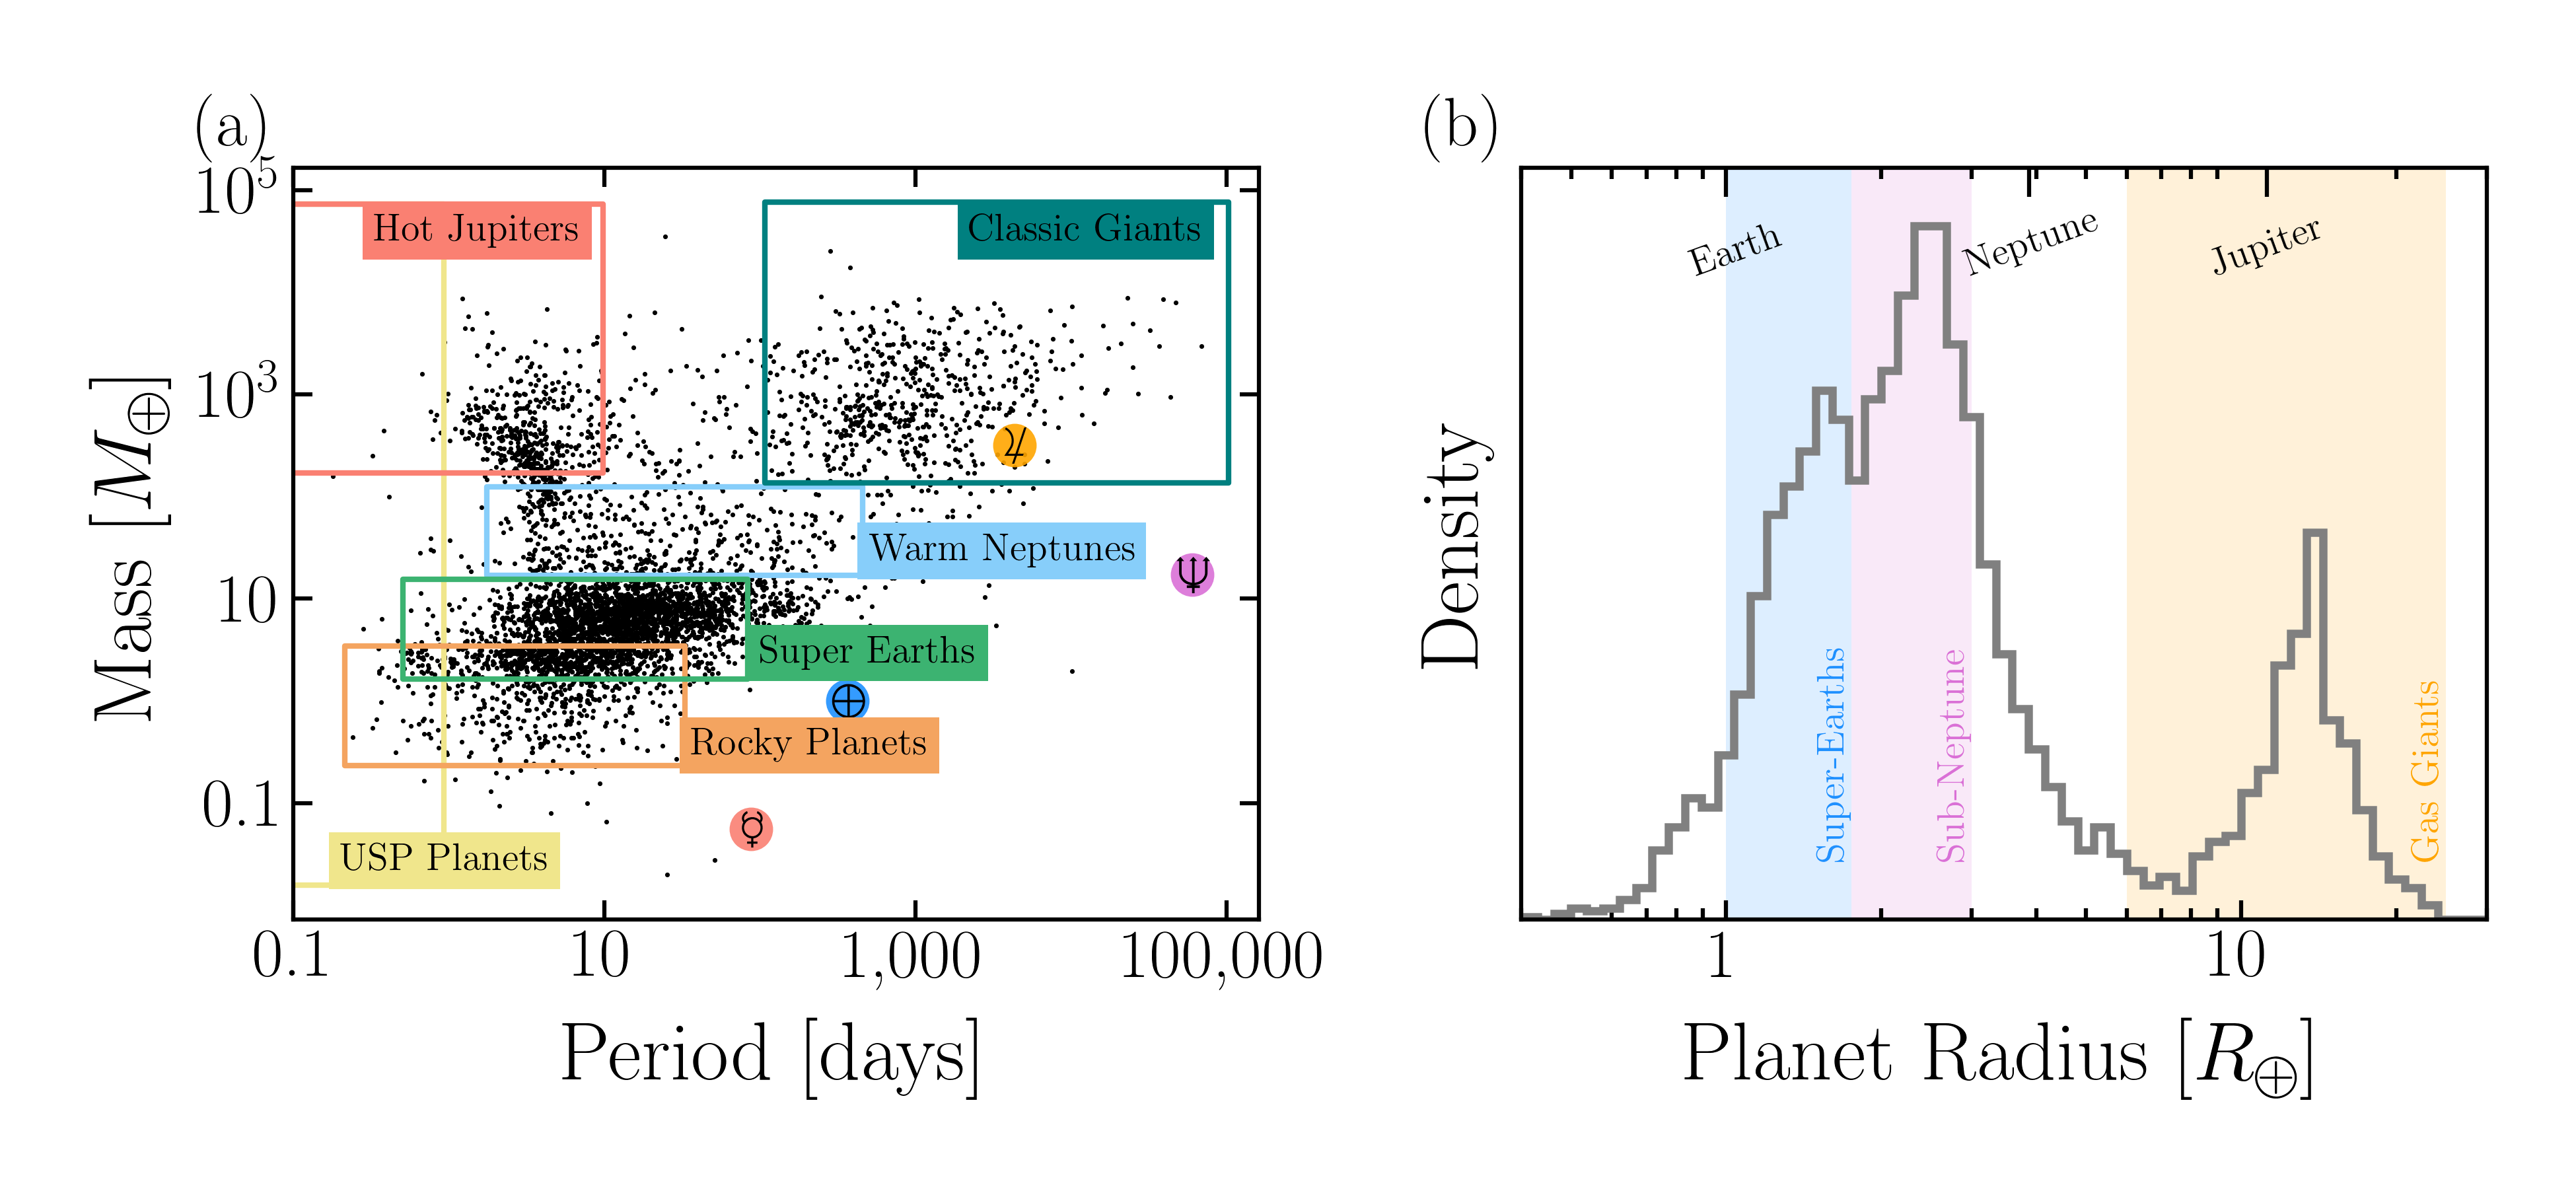
\includegraphics[width=1.1\linewidth]{src/figures/scatter_categories.png}}
  \caption{\textbf{Exoplanet Categories:} (Right) Scatter plot of confirmed exoplanet masses on the vertical axis and orbital periods on the horizontal axis. (Left) Histogram of confirmed exoplanet radii. The symbols are shorthand for solar system planets:  Mercury ($\Mercury$), Earth ($\Earth$), Neptune ($\Neptune$), and Jupiter ($\Jupiter$). 
  Data has been obtained from \href{https://exoplanetarchive.ipac.caltech.edu/}{\textsc{ExoFop}}. \github{https://github.com/avivajpeyi/exoplanet_catalog_plotter}}
  \label{fig:exo_categories}
\end{center}
\end{figure}



\paragraph{Big to small:}
Before Kepler's launch, most exoplanets identified (using radial velocity) were hot, massive gas giants, top region of Figure~\ref{fig:exo_categories}a~\cite{kepler_mission}.
These large planets were so close to their host stars that they caused a pronounced ``wobble'' in the stellar spectra, making them stand out in radial velocity exoplanet searches~\cite{kepler_mission}.
Therefore, estimating  the proportion of terrestrial (planets with radii $R\sim1-3\ R_{\oplus}$)  and Jovian planets  ($R\sim10-20\ R_{\oplus}$) was one of Kepler's primary objectives.

Kepler was successful in this mission as its data revealed many Jovian and terrestrial planets, both found via the transit method~\cite{kepler_mission}.
Figure~\ref{fig:exo_categories}b shows that there are a far greater number of small exoplanets (radii less than Neptune's) than the giant exoplanets (radii above Neptune's).
The most common planets have radii in the super-Earth and sub-Neptune categories. 
This makes our solar system rather peculiar: the most common types of planets in the Galaxy are completely absent from our solar system and were unknown until Kepler’s survey~\cite{Oppenheimer:2016:Sci}.

The region between the super-Earths and sub-Neptunes in Figure~\ref{fig:exo_categories}b also contains an interesting gap, called the photoevaporation valley (also known as the Fulton gap)~\cite{Owen:2013:ApJ, VanEylen:2018:MNRAS}. 
This valley occurs due to atmospheric stripping of 1.5-2 $M_{\oplus}$ planets, leaving a population of stripped, rocky planets close to their stars (the super-Earths). 
The planets that avoid stripping form a second population of thick-atmosphere planets farther away from their stars (the sub-Neptunes)~\cite{VanEylen:2018:MNRAS}.

It is important to note that even the transit approach with Kepler data has biases — it has trouble finding planets with radii $R<R_{\oplus}$ and lengthy periods~\cite{kepler_mission}.
The dearth of small-sized long-period planets can be seen in the bottom right side Figure~\ref{fig:exo_categories}a.


\begin{figure}
\begin{center}
  \centerline{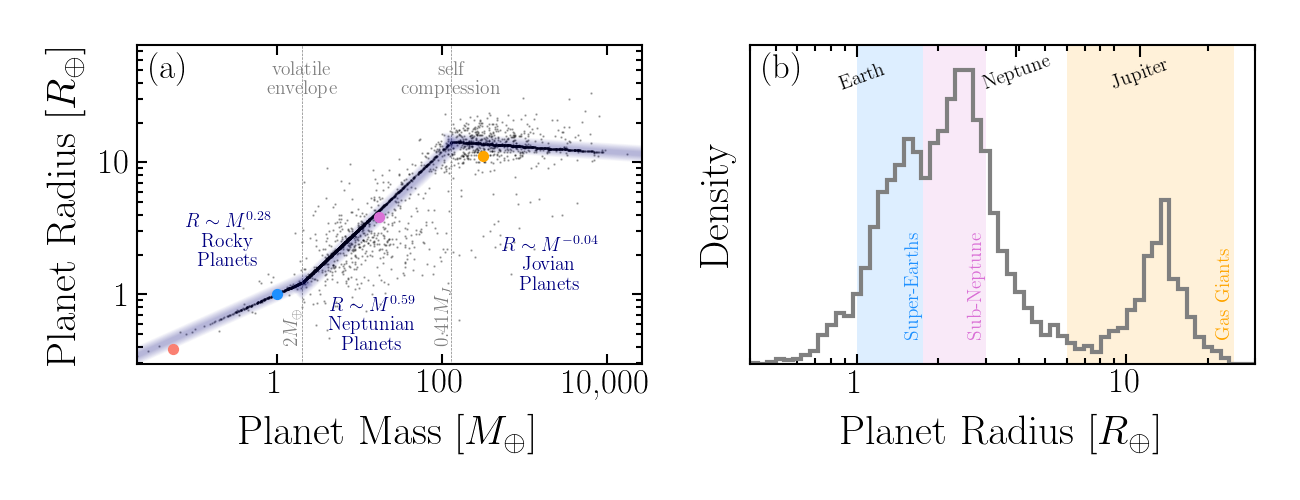
\includegraphics[width=1.1\linewidth]{src/figures/radii_and_mass_relations.png}}
  \caption{\textbf{Searching for habitable exoplanets:} 
  (Left) Scatter plot of confirmed exoplanet radii on the vertical axis and masses on the horizontal axis. The purple shaded curve represents the best-fit mass radius power-laws from \citet{Chen:2017:ApJ}. (Right) Scatter plot of confirmed exoplanet host star masses on the vertical axis and the exoplanet distance from their stars on the horizontal axis.
  Habitable zone data plotted in green, obtained from and work by \citet{Kopparapu:2014:ApJL}. 
  The symbols $\Mercury$, $\Earth$, $\Neptune$, and $\Jupiter$ stand for Mercury, Earth, Neptune, and Jupiter. 
  Exoplanet data has been obtained from \href{https://exoplanetarchive.ipac.caltech.edu/}{\textsc{ExoFop}}. 
  \github{https://github.com/avivajpeyi/exoplanet_catalog_plotter}}
  \label{fig:exo_mass_radius_relations}
\end{center}
\end{figure}


\paragraph{Looking for signs of life:}
In addition to identifying different-sized planets, Kepler's mission was designed to investigate habitable worlds~\cite{kepler_mission}.
Scientists define habitable worlds as solid planets with a wide enough orbit to form liquid water on their surface (the star's habitable zone).
This section discusses these two conditions.

Density estimates can indicate if the planet is solid.
By estimating exoplanet masses (using radial velocity measurements) and radii (using the transit method), scientists can compute the density and infer whether a planet is composed primarily of rock, water, or gas.
The mass and radii of planets are plotted in Figure~\ref{fig:exo_mass_radius_relations}a. 
Planets with masses below $2\ M_{\oplus}$ (or $R < 1.23 R_{\oplus}$) are termed \textit{Rocky/Terran worlds} due to their rocky, Earth-like composition (e.g., Earth, Mercury, Venus, Mars)~\cite{Oppenheimer:2016:Sci}.
Next are the \textit{Neptunian worlds}, which have a gaseous ``volatile envelope'' (e.g. Saturn, Uranus, and Neptune)~\cite{Chen:2017:ApJ}.
The final group consists of gas giants, or \textit{Jovian worlds} (e.g. Jupiter).
Figure~\ref{fig:exo_mass_radius_relations}a shows that additional mass increases the radii of terrestrial and Neptunian planets, but decreases the size of gas giants due to ``self-compression" by gravity.
Using planets with mass and radius measurements, scientists constructed a mass-radius power-law relation, represented in Figure~\ref{fig:exo_mass_radius_relations}a by the broken purple power-law~\cite{Chen:2017:ApJ}.
This power-law was utilized to deduce mass/radius predictions for planets with a radius/mass measurement — the dense cluster of planets in the centre of the purple power-law~\cite{Chen:2017:ApJ}.
In turn, the mass and radii of numerous exoplanets have suggested a population of rocky planets~\cite{kepler_mission}.
However, the question of if the planets are within the habitable zone is more complex.


Initial theory suggested that a star's habitable zone (HZ) is a function of its mass. 
However, improved models demonstrate the importance of incorporating a myriad of additional parameters like planetary rotation~\cite{Yang:2014:ApJL},  mass~\cite{Kopparapu:2014:ApJL}, albedo, atmospheric heating~\cite{Kasting:2011:AsBio}, and others~\cite{Yang:2014:ApJL, Kopparapu:2013:ApJ, Kopparapu:2014:ApJL, Shields:2014:ApJL}. 
Plotted in Figure~\ref{fig:exo_mass_radius_relations}b is \citet{Kopparapu:2014:ApJL}'s (slightly outdated) habitable zone fit, containing over 250 exoplanets.
Although not all of these planets in the HZ will truly be habitable, these planets act as potential candidates for future follow-up. 
Furthermore, recent work by 
\citet{Bryson:2021:AJ} combining Kepler exoplanet data with Gaia stellar data estimated that our galaxy contains over 3 hundred-million potentially habitable planets.
Hence, there should be more than just 250 habitable exoplanet candidates.


\subsection{Passing the baton from Kepler to TESS }
As seen in the preceding sections, Kepler's mission was a tremendous success and led to the discovery of thousands of exoplanets.
However, the Kepler mission was not devoid of difficulties.
The mission ran into issues when two of the four reaction wheels failed (required for precise alignment). 
This malfunction concluded Kepler's primary mission in 2013~\cite{cowen2013wheels}.
Kepler continued to operate until its fuel ran out in 2018~\cite{KeplerShutdown}.\footnote{The command ``goodnight'' triggered Kepler's shutdown on November 15, 2018. This date coincides with Johannes Kepler's death anniversary~\cite{KeplerShutdown}.}

A few months after, TESS, the Transiting Exoplanet Survey Satellite, replaced Kepler as the primary spacecraft to discover new exoplanets.
While Kepler surveyed less than 1\% of the sky, TESS has surveyed over 75\% of the sky and will get full coverage over the next few years~\cite{tess}. 
Additionally, TESS observes brighter stars than Kepler to enable follow-up on some exoplanets via ground-based telescopes.  
So far, TESS has found over $\sim250$ confirmed planets and has over $\sim6,000$ candidate exoplanets~\cite{Akeson:2019:AAS,  Stassun:2019:AJ}. 
To aid in promoting some of these candidates to confirmed planets, we analyze all the candidates with a Bayesian inference framework. 
This work is presented in Chapter~\ref{ch.tess}.


\section{Thesis Overview}
The remaining sections of the dissertation are organised as follows. 
\cref{ch.bcr} presents a Bayesian-inspired ranking statistic to aid in the search for gravitational waves from intermediate-mass black holes. 
A review of alternative methods for detecting IMBHs is presented in \aref{apdx.imbh}. 
\cref{ch.pbilby} introduces a parallelized nested sampling library for gravitational wave parameter estimation. 
This covers the parameter estimation method and software utilised in subsequent gravitational wave chapters. 
\cref{ch.deep} documents a new method for resolving inconsistencies between two sets of opposing posteriors. 
The method is demonstrated with an analysis of GW151226. 
\cref{ch.agn} introduces a phenomenological model for ensemble spin properties of black holes in AGNs. It estimates the number of observations required for the model to constrain AGN parameters. 
\cref{ch.tess} presents an updated catalogue of candidate exoplanet parameters estimated from Bayesian inference, demonstrating the versatility of Bayesian methods outside of gravitational waves.
\cref{cp.conc} concludes with remarks on the future of gravitational waves and exoplanet research.
